% main_v10_author_prose.tex
% v10 LaTeX shell. Article prose to be supplied by author/editor.
% Evidence/data inserts: see v10_data_pack.md (same directory).
% Do NOT add prose, scaffolding labels, table of contents, or front-matter
% non-claim blocks to this shell. Wait for author-supplied text.
%
\documentclass[11pt,a4paper]{article}

\usepackage[utf8]{inputenc}
\usepackage[T1]{fontenc}
\usepackage{lmodern}
\usepackage{amsmath,amssymb,amsthm}
\usepackage{graphicx}
\usepackage{booktabs}
\usepackage{xcolor}
\usepackage[margin=1in]{geometry}
\usepackage[hidelinks]{hyperref}
\usepackage{caption}
\usepackage{microtype}
\usepackage{textcomp}
\usepackage{placeins}
\usepackage{tikz}
\usetikzlibrary{arrows.meta,shapes.geometric,shapes.misc,positioning,calc}

\newtheorem{theorem}{Theorem}
\newtheorem{conjecture}{Conjecture}
\newtheorem{definition}{Definition}
\newtheorem{lemma}{Lemma}

% Final-layout pass: absorb the single sub-6.5pt overfull line in §2
% without altering prose. Activates only on otherwise-overfull lines.
\setlength{\emergencystretch}{1em}

\title{A Stress-Energy-First Finite Audit Framework for\\
       Positive-Energy Warp-Shell Geometries:\\
       \large Boxed LP Certificates, Reduced-Operator Sensitivity and Source-Realisation Gates}
\author{Onur Alexander William Aydogan\\
        Waynestark Enterprises Limited}
\date{}

\begin{document}

\maketitle

\begin{abstract}
A warp-shell metric can be written down before one knows whether any physical source can produce it. In general relativity this is not a minor omission: the source must be a stress-energy tensor that is conserved, positive in the relevant energy-condition sense, finite in total ledger energy, stable as a constitutive system, and compatible with a matter model. This paper studies the corresponding source-side problem for positive-energy warp-shell geometries. We define an admissible class $A_{+}$, remove response channels targeted by matched-control template surrogates, and formulate the continuum target $C[T]$, which motivates two mathematically distinct finite constructions without evaluating the continuum supremum.

The audit uses two distinct finite constructions. First, a boxed finite-audit linear programme with its Karush--Kuhn--Tucker (KKT) dual certificate closes at $C_{\mathrm{LP}}^{(N,B,\Omega)}=5.826$ for a single matched-control-orthogonal response observable over the finite audit class $A_{\mathrm{audit},N,B,\Omega}$; this value is cap-dependent (the coefficient-box-inactive optimum under the remaining constraints is $\approx13.07$), not a continuum bound. The finite programme imposes conservation, moment closure, a density cap, coefficient box bounds and sampled linear stress-cone surrogate inequalities; these rows are motivated by energy-condition structure but are not exact covariant NEC/WEC/DEC tests. A pointwise check confirms the surrogate status --- at the LP optimum only a minority of sampled cells satisfy the exact covariant energy conditions --- so ``positive-energy'' here names the Bobrick--Martire background geometry class, not the audited optimum. Second, a separate reduced-operator spectral model, calibrated to a finite-band anchor $A_{\mathrm{HT}}=6.39$, produces box-independent spectral ratios $r_{S}$; the clean sequential ratio $r\simeq3.3146$ gives the calibrated reduced-operator index $I_{\mathrm{clean}}\simeq21.18$. The reduced indices $I_{S}$ are calibrated spectral-norm sensitivity values --- not linear-programme optima, not KKT-certified, and not proved equal to $C_{\mathrm{LP}}$. The topological-containing precursors $13.41$ and $26.12$ are retained only as provenance; the higher candidates $59.81$ and $133.99$ are partial and speculative.

At fixed compactness $u=0.20$ and under an explicit illustrative scale mapping $I_{S}R^{2}=10^{6}\,\mathrm{km}^{2}$ (a stated normalisation, not a relation derived from the audit), the clean reduced index maps to $R\simeq217.3\,\mathrm{km}$, $M\simeq29.4\,M_{\odot}$ and reconstructed peak density $\rho_{\mathrm{peak}}\simeq3.5\times10^{15}\,\mathrm{kg\,m^{-3}}$; these values are conditional on the $6.39$ anchor and the scale constant. The ordinary isotropic equation-of-state/Tolman--Oppenheimer--Volkoff (TOV) comparison, materials, operations and standards gates all fail. The result is a reproducible stress-energy-first finite-audit framework together with a matter-realisation obstruction on the audited class --- not a warp-drive construction, a universal no-go theorem, or a fully GR-derived response bound.
\end{abstract}

%-----------------------------------------------------------
\section{Introduction}\label{sec:intro}
%-----------------------------------------------------------

A spacetime metric is not the same thing as a physical source. In general relativity the metric $g_{\mu\nu}$ determines curvature, but the curvature must be supplied by a stress-energy tensor through Einstein's equation,
\[
G_{\mu\nu}=8\pi G\,T_{\mu\nu}.
\]
One may always read this equation algebraically from right to left or left to right. Given a smooth metric, one can formally define $T_{\mu\nu}=G_{\mu\nu}/(8\pi G)$. The difficulty is that such a tensor need not be a physically admissible source. It may fail covariant conservation, violate the null, weak or dominant energy conditions, require uncounted auxiliary reservoirs, lack a stable constitutive closure, or sit outside any equation of state capable of supporting the required density and pressure. This distinction is elementary, but in warp-shell discussions it is often the point at which a geometric construction ceases to be a source model. \cite{Wald1984,HawkingEllis1973}

Recent positive-energy warp-shell work, beginning with Bobrick and Martire and followed by constant-velocity and numerical-relativity studies, has clarified the geometry-side problem. Bobrick and Martire introduced a physical-warp-drive framework in which positive-energy, \emph{subluminal} configurations can be discussed without the original Alcubierre negative-energy shell; Fuchs et al.\ supplied an explicit constant-velocity subluminal solution satisfying the energy conditions. By contrast, Clough, Dietrich and Khan study the numerical-relativity collapse of an NEC-violating Alcubierre-type configuration with an assumed stiff equation of state, which is not a positive-energy continuation of that sequence. Observer-independent analysis (Santiago, Schuster and Visser) further shows that generic physically reasonable warp drives violate the null energy condition when the requirement is imposed for all observers. Two recent unrefereed preprints by Le are relevant to future scope rather than to the present result: an eigenstructure-based, observer-robust energy-condition test, which bears directly on the finite observer sample used here, and a causal, subluminal radiative-recoil steering construction, which lies outside the present stationary reduced-operator audit; both are treated here as recent methodological developments, not settled authority. These advances sharpen the source-side question: if a warp-shell geometry can be represented as initial data or as a candidate metric, what stress-energy source would actually realise it? The gap addressed here is different: whether an admissible stress-energy source can generate a bounded residual response once the channels targeted by the matched-control template surrogates are removed. \cite{BobrickMartire2021,Fuchs2024,CloughDietrichKhan2024,SantiagoSchusterVisser2022,Le2026ObserverRobust,Le2026Steering}

This paper answers a narrower question than buildability. We ask how large the residual warp-shell response can be, per unit total energy, after subtracting the channels targeted by the matched-control template surrogates. Boundary data, gauge effects, asymptotic flux and memory, and cross-channel energy transfers are not counted as novel source response. They are projected out. What remains is a channel-identity residual: the part of the response that cannot be attributed to the matched-control suite.

The construction proceeds in three stages. First, we define an admissible source class $A_{+}$ of stress-energy tensors satisfying conservation, pointwise energy conditions, finite total ledger energy, no horizon or trapped surface on the audited slices, and stable causal constitutive closure. We then linearise the source-to-metric response by an operator $K$, remove matched controls by $Q=I-P_{\mathrm{controls}}$, and normalise the projected response to obtain
\[
C[T]=
\frac{c^{4}R}{G\,E_{\mathrm{total}}[T]}\,
\bigl\| Q K T \bigr\|_{W}.
\]
The quantity $C[T]$ is the continuum target concept. The present paper does not evaluate this continuum supremum directly; it constructs one finite scalar LP certificate and one separate reduced spectral model. As a concept $C[T]$ is a dimensionless response coefficient on a source class, not a speed, not a thrust, and not a device performance.

Second, we compute the boxed finite-audit LP certificate $C_{\mathrm{LP}}$ in the fixed-operator problem. Holding $K$, $Q$ and $W$ fixed, the optimisation over the finite admissible polyhedron becomes a boxed finite linear programme. Operationally, the calculation replaces the continuous source tensor by a finite coefficient vector $x$, imposes the implemented linear constraints --- conservation and moment closure (equalities), and sampled stress-cone surrogate inequalities, a density cap and coefficient box bounds (inequalities) --- and maximises the discretised response functional $\ell^{\top}x$. The finite inequality rows are sampled linear surrogates motivated by the energy conditions, not exact covariant NEC/WEC/DEC tests, and the full energy ledger, no-horizon and constitutive-stability requirements remain continuum goals of $A_{+}$ that this LP does not implement. The reported value is certified because the primal optimum and the dual upper bound coincide to numerical precision. At the audited baseline discretisation this gives $C_{\mathrm{LP}}=5.826$. A high-truncation finite-band correction gives $A_{\mathrm{HT}}=6.39$, and the same value appears as the finite-band spectral upper bound $U\leq6.39<100$. A passive Kramers--Kronig argument suggests a higher heuristic spectral-weight estimate $C_{\mathrm{passive}}=583$. That value is not used as the working-envelope bound, because the sharp passive coefficient, the extension to arbitrary stationary admissible backgrounds, and the finite-band dispersion trade-off remain open. The exploratory working benchmark carried by the paper is therefore $C_{\mathrm{work}}=10^{4}$ (an adopted benchmark, not a proved inequality or upper bound).

Third, we admit controlled operator-side variations and compute reduced spectral-response ratios $r_{S}$ and calibrated indices $I_{S}=A_{\mathrm{HT}}r_{S}$. Here a case means a numerical index together with its model-input status. A joint reduced-operator composition gives $I_{\mathrm{joint,prov}}=13.41$ and a sequential reduced-operator composition gives $I_{\mathrm{seq,prov}}=26.11858$ (rounded to $26.12$); both include a topological factor whose mechanism carries an adversarial KILL verdict. Removing it gives the clean joint $I_{\mathrm{joint,clean}}\approx10.44$ and the clean retained value $I_{\mathrm{seq,clean}}\approx21.18$, which are the values carried forward in this audit, with $13.41$ and $26.12$ preserved as provenance. Two higher outputs are recorded but not retained: $I_{\mathrm{partial}}=59.81$, because it depends on two Tier-2 estimate-only mechanism factors, and $I_{\mathrm{spec}}=133.99$, because it depends on a regularised extremiser candidate with an unresolved provenance and stability risk. The distinction between retained, partial and speculative values is part of the result.

The retained reduced-operator index is still not a source. To give it physical scale, we use the audit-chain scale convention $I_{S}R^{2}=10^{6}\,\mathrm{km}^{2}$ at fixed compactness
\[
u=\frac{GM}{c^{2}R}=0.20.
\]
For the clean value $I_{\mathrm{seq,clean}}\approx21.18$, this scale convention gives a scale-convention reconstruction $R\simeq217.3\,\mathrm{km}$ and $M\simeq29.4\,M_{\odot}$. The corresponding surface escape-velocity ratio is $v_{\mathrm{esc}}/c=\sqrt{2u}\simeq0.6325$, and the reconstructed peak source density is $\rho_{\mathrm{peak}}\simeq3.5\times10^{15}\,\mathrm{kg\,m^{-3}}$. These are compact-object-scale conditions, not engineering-material conditions.

The matter-side audit then fails at every gate tested. No audited isotropic static equation of state closes the Tolman--Oppenheimer--Volkoff (TOV) system at the required mass-radius pair. The material catalogue, including ordinary structural materials, dense auxiliary metals, high-stiffness metamaterial candidates and ML-generated material candidates, remains around $10^{3}$ to $10^{4}\,\mathrm{kg\,m^{-3}}$, leaving a factor of $10^{11}$ to $10^{12}$, or 11 to 12 orders of magnitude, against the retained-rung peak density. Operations at $u=0.20$ fall outside ordinary station-keeping and proximity envelopes. The audited NASA, ECSS and GSFC standards bundle, supplemented by Failure Modes and Effects Analysis (FMEA) and Fault Tree Analysis (FTA), qualifies support and auxiliary hardware only; it has no recognised category for compact-object source matter.

The conclusion is deliberately limited. The paper does not construct a warp drive, does not exhibit a buildable source, and does not claim that the selected clean calibrated index is a propulsion speed. It gives a finite-audit operator-side response certificate on a defined admissible class, records the certification status of higher candidates, and shows that the retained rung fails the source-realisation gates presently available. Extensions beyond $A_{+}$, including non-passive response, modified gravity, energy-condition violation, or fully dynamical three-dimensional numerical-relativity branches, are outside the claim.

%-----------------------------------------------------------
\section{Source-side formulation}\label{sec:formulation}
%-----------------------------------------------------------

The source-side problem begins with a restriction. We do not treat every algebraic rearrangement of Einstein's equation as a physical source. A candidate source must also pass conservation, energy-condition, energy-ledger, horizon and constitutive-stability tests. We optimise over stress-energy tensors that satisfy a defined set of physical admissibility tests. The purpose of this section is to specify that set, describe the response map from source perturbation to metric perturbation, and define the dimensionless coefficient $C[T]$ whose bound is computed later.

\subsection{The admissible source class}

Let $(M,\bar{g}_{\mu\nu})$ be the audited positive-energy warp-shell background. We keep $G$ and $c$ explicit and use signature $(-,+,+,+)$. The geometric aperture of the source is denoted by $R$, and the compactness used for the later scale ledger is
\[
u=\frac{GM}{c^{2}R}.
\]
The audit evaluates the retained physical scale at $u=0.20$, but the definition of the source class itself does not depend on a particular numerical value of $u$.

We denote by $A_{+}$ the class of stress-energy tensors $T_{\mu\nu}$ satisfying the following five conditions:
\[
\nabla_{\mu}T^{\mu\nu}=0,
\]
the pointwise null, weak and dominant energy conditions hold for admissible observers, the total energy ledger $E_{\mathrm{total}}[T]$ is finite after summing all declared matter, field, auxiliary and control reservoirs, the audited spacelike slices contain no horizon or trapped surface, and the constitutive closure is stable and causal. The last condition excludes source models whose apparent response comes from ghosts, tachyonic modes, or unstable constitutive equations rather than from admissible stress-energy.

The energy conditions and conservation law are standard source-side requirements in classical relativity and semiclassical settings. The ledger condition is more specific to the present audit. It prevents an apparent enhancement from being counted in one channel while the energy required to create, support, or control that channel is hidden elsewhere. A field reservoir, control reservoir, supporting structure, or auxiliary system is therefore part of the denominator if it is part of the proposed source.

This definition is deliberately narrower than all conceivable ways of modifying a warp-shell geometry. It excludes bulk negative-energy matter, non-passive response branches, modified-gravity changes to Einstein's equation, and fully dynamical three-dimensional numerical-relativity configurations outside the audited stationary baseline. Those exclusions are not denied possibilities. They are outside the class bounded in this paper.

\subsection{Linear response and matched controls}

For a source perturbation $T_{\mu\nu}\in A_{+}$, the linearised metric response is written
\[
h_{\mu\nu}[T] = K_{\mu\nu}{}^{\alpha\beta}\,T_{\alpha\beta},
\]
where $K$ is the response operator on the audited background. The details of $K$ depend on the background, gauge and finite-band truncation, but the role of $K$ is simple: it maps an admissible source perturbation to the corresponding linearised metric response.

The full response $KT$ is not the quantity we want to count. Some pieces of the response are represented by matched-control template surrogates --- constructed to stand in for boundary-data, gauge, asymptotic-flux, memory, and cross-channel-ledger contributions, motivated by ordinary general relativity but not derived from it. Counting those pieces as novel warp-shell response would overstate the result. We therefore introduce a matched-control projector $P_{\mathrm{controls}}$, and define
\[
Q=I-P_{\mathrm{controls}}.
\]
The projected response $QKT$ is the channel-identity residual. It is the part of the response left after subtracting the matched-control suite.

The matched controls include positive-mass boundary-data controls, gauge controls, asymptotic-data and memory controls, and cross-channel ledger controls. Positive-mass boundary data are controlled using the standard positive-mass structure. Gauge controls remove coordinate artefacts. Asymptotic and memory controls remove flux and displacement-memory contributions associated with the asymptotic symmetry description. Ledger controls prevent the same energy movement from being counted as source response in one channel and as unpaid support in another. \cite{SchoenYau1981,Witten1981,Strominger2014,WaldIyer1990}

The control suite is frozen for the audit. A leave-one-template-out and random-subspace sensitivity test shows $C_{\mathrm{LP}}$ changes by at most about $\pm8\%$ under control-suite variations, and random suites give slightly \emph{higher} $C_{\mathrm{LP}}$ (consistent with the physical templates subtracting more response), so the certificate is a property of the chosen template surrogates to that tolerance. Enlarging it would not make the reported bounds weaker in the sense of creating a larger novel response; it would subtract more ordinary or already-accounted response and could only sharpen the residual. The coefficient below is therefore always a coefficient for the projected residual, not for the total metric perturbation.

\subsection{The response coefficient}

The projected response is measured in a weighted norm $\|\cdot\|_{W}$ supported on the matched-control-orthogonal subspace. We normalise by the full energy ledger and by the gravitational aperture scale to define
\[
C[T] = \frac{c^{4}R}{G\,E_{\mathrm{total}}[T]}\,\bigl\| Q K T \bigr\|_{W}.
\]
The factor $c^{4}R/G$ has dimensions of energy, so $C[T]$ is dimensionless. The coefficient measures how much matched-control-orthogonal warp-shell response is obtained per unit total ledger energy, expressed in units natural to the gravitational aperture. Here $K$ is the audited finite-band linear response operator, $Q=I-P_{\mathrm{controls}}$ is the matched-control subtraction operator used in this audit, and $W$ is the chosen weighted norm. These are the operative definitions used by the finite audit; a full continuum statement would require explicit operator definitions together with the truncation-error and polyhedron-approximation control noted in §3.

\begin{figure}[ht]
\centering
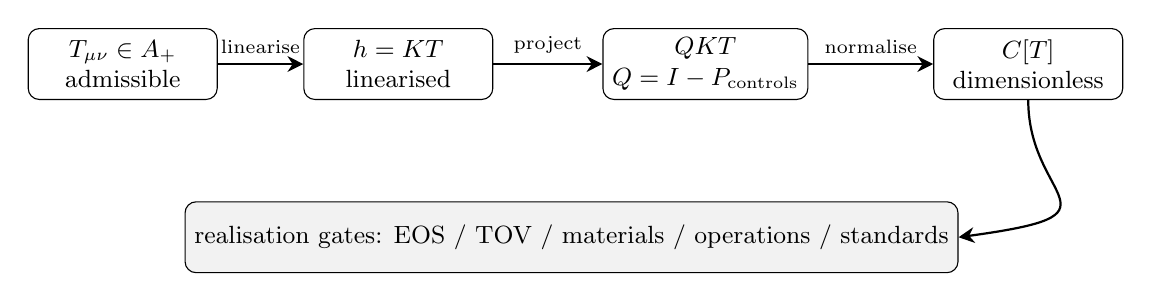
\begin{tikzpicture}[
  every node/.style={font=\small},
  box/.style={draw, rounded corners, minimum width=2.4cm, minimum height=0.9cm, align=center},
  arr/.style={-{Stealth[length=2mm,width=2mm]}, thick},
]
\node[box] (T) at (0,0) {$T_{\mu\nu} \in A_{+}$\\admissible};
\node[box] (h) at (3.5,0) {$h = K T$\\linearised};
\node[box] (Q) at (7.4,0) {$QKT$\\$Q = I - P_{\mathrm{controls}}$};
\node[box] (C) at (11.5,0) {$C[T]$\\dimensionless};
\node[box, fill=gray!10] (G) at (5.7,-2.2) {realisation gates: EOS / TOV / materials / operations / standards};
\draw[arr] (T) -- node[above, font=\scriptsize]{linearise} (h);
\draw[arr] (h) -- node[above, font=\scriptsize]{project} (Q);
\draw[arr] (Q) -- node[above, font=\scriptsize]{normalise} (C);
\draw[arr] (C.south) .. controls +(0,-1.3) and +(2.2,0.3) .. (G.east);
\end{tikzpicture}
\caption{Stress-energy-first formulation. An admissible source $T_{\mu\nu}\in A_{+}$ is mapped by the linearised response operator $K$, projected by $Q=I-P_{\mathrm{controls}}$, and normalised by the full energy ledger to form $C[T]$. The matter-realisation gates are applied separately; passing the operator-side bound does not imply EOS, material, operational or standards realisation.}
\label{fig:flow}
\end{figure}

This normalisation is the reason $C[T]$ is not a speed. It should therefore be read as a response-per-energy coefficient on $A_{+}$, not as a trajectory, speed or travel-time model. A large value of $C[T]$ would mean that an admissible source produces a large projected residual response for its total ledger energy. It would not, by itself, show that the source can be realised as matter.

The continuum target for a future physical audit is the supremum of $C[T]$ over the admissible class; the present paper does not evaluate this continuum quantity, and instead studies two finite constructions related to it:
\[
C_{\mathrm{max}} = \sup_{T \in A_{+}} C[T].
\]
\subsection{Three distinct audited objects}

The continuum target $C[T]$ is not evaluated directly. Two \emph{different} finite constructions are used, and they must not be conflated. First, a boxed finite-audit linear programme. After finite-band truncation an admissible source is a dimensionless coefficient vector $\tau=t/\varepsilon_{S}\in\mathbb{R}^{N}$ ($\varepsilon_{S}$ the fixed stress-energy scale, $t$ the dimensional coefficient), and the certified quantity is
\[
C_{\mathrm{LP}}^{(N,B,\Omega)} = \max_{\tau\in A_{\mathrm{audit},N,B,\Omega}} \ell^{\top}\tau,
\]
where the finite audit class is
\[
A_{\mathrm{audit},N,B,\Omega}=\bigl\{\tau\in\mathbb{R}^{N}: A_{\mathrm{eq}}\tau=0,\ A_{\mathrm{ineq}}(\Omega)\tau\le b_{\mathrm{ineq}},\ -B\mathbf{1}\le\tau\le B\mathbf{1}\bigr\}.
\]
Here $\ell$ is the discretised, matched-control-orthogonalised (via $Q_{\mathrm{LP}}$) response vector of a single fixed scalar observable, the \texttt{delta\_H} holonomy channel: the low-multipole Sagnac-type response kernel $K_{\Delta H}(x)=G/(c^{4}R_{\mathrm{loop}}\,d(x))$ (with $d(x)=|x|+R_{\mathrm{reg}}$) evaluated over the audited cells and projected onto the finite basis --- it measures the loop-holonomy sensitivity of the shell aperture to the admissible source. Thus $\ell^{\top}\tau$ is a support functional, \emph{not} a Euclidean norm; $N=2880$ is the coefficient dimension at radial resolution $N_{r}=32$; $B=1.5$ is the coefficient-box half-width (a numerical scaling cap, distinct from the physical density cap); $\Omega$ is the finite observer sample entering the energy-condition rows. The equality block ($128$ rows) imposes conservation and moment closure; the inequality block ($23809$ rows) imposes the sampled stress-cone surrogate inequalities (NEC-, WEC- and DEC-inspired; stated explicitly below) on $\Omega$, the density cap and the positivity row. The class $A_{+}$ is the intended continuum, all-observer source class; $A_{\mathrm{audit},N,B,\Omega}$ is the finite sampled set actually certified; its rows are surrogate constraints, so membership does not prove membership in the exact continuum positive-energy class $A_{+}$. The Karush--Kuhn--Tucker certificate applies only to this finite polyhedron; no continuum convergence, covariant energy-condition satisfaction, or all-observer equivalence is proved. The observer sample $\Omega$ comprises $12$ deterministic Fibonacci-sphere unit vectors $n$ in one coefficient frame. For each $n$ the finite matrix imposes the coded linear surrogates $\rho+n\!\cdot\!S+n\!\cdot\!P\!\cdot\!n\ge0$, $\rho\ge0$, $\rho\pm n\!\cdot\!S\ge0$ and $|n\!\cdot\!P\!\cdot\!n|\le\rho$, with $n\!\cdot\!P\!\cdot\!n=\sum_{i}n_{i}^{2}P_{ii}+2\sum_{i<j}n_{i}n_{j}P_{ij}$ and component ordering $(\rho,S_{x},S_{y},S_{z},P_{xx},P_{yy},P_{zz},P_{xy},P_{xz},P_{yz})$ (here $S$ denotes the momentum-density components $T_{0i}$ and $P$ the spatial stress $T_{ij}$, off-diagonals entering $n\!\cdot\!P\!\cdot\!n$ with the factor $2$ shown). These are \emph{sampled stress-cone surrogate inequalities}: they are not exact covariant NEC, WEC or DEC contractions (no metric or observer four-velocity is formed), and satisfying them does not establish the physical energy conditions for the sampled or for all observer four-velocities. A row-by-row audit reproduces the frozen $A_{\mathrm{ineq}}$ rows to machine precision (Appendix~\ref{app:provenance}). Only this single coefficient frame is sampled, so no observer-robust energy-condition result is claimed; observer-robust implementation is a defined future work package. The normalisation scale $\varepsilon_{S}=7.747\times10^{24}\,\mathrm{J\,m^{-3}}$ is an energy-density scale: the generator carries the $\rho$-component as an energy density $T^{00}$ and never divides by $c^{2}$. It fixes the dimensionless coefficient $\tau=t/\varepsilon_{S}$. The density-cap row is dimensionally $\Phi(\rho\text{-coeffs})\le\varepsilon_{S}$; after normalisation the dimensionless cap on the $\rho$-component is $1$ (the frozen $b_{\mathrm{ineq}}$ cap entry is exactly $1$, in $\tau$-space). The corresponding mass-density scale is $\varepsilon_{S}/c^{2}$; the physical peak-density reconstruction ($\approx3.5\times10^{15}\,\mathrm{kg\,m^{-3}}$) comes from the separate scale mapping, not from $\varepsilon_{S}$ directly. The implemented finite constraint set contains conservation, moment closure, the sampled stress-cone surrogate inequalities, the density cap and coefficient box bounds only; it does \emph{not} implement the full energy ledger, no-horizon, constitutive-stability or ghost/tachyon exclusions, which are continuum admissibility goals of $A_{+}$ not certified by this LP. Second, a reduced-operator spectral model on a $32$-dimensional radial grid, which measures singular-value ratios $r_{S}=\sigma_{\max}(Q_{\mathrm{red}}K_{S})/\sigma_{\max}(Q_{\mathrm{red}}K_{0})$ under controlled operator compositions and converts them to calibrated indices $I_{S}=A_{\mathrm{HT}}\,r_{S}$, $A_{\mathrm{HT}}=6.39$. Its projector $Q_{\mathrm{red}}$ and the baseline projector $Q_{\mathrm{LP}}$ are different operators (Appendix~\ref{app:operators}); equivalence of $C_{\mathrm{LP}}$ and $I_{S}$ is not proved.

Section 3 computes the boxed LP certificate with $K$, $Q_{\mathrm{LP}}$, and $W$ held fixed. Section 4 then asks what happens when controlled operator-side variations are admitted. Section 5 returns to the physical question postponed by the optimisation: whether the selected clean calibrated index corresponds to any matter source that can pass the equation-of-state, TOV, materials, operations and standards gates.

%-----------------------------------------------------------
\section{Boxed finite-audit LP certificate}\label{sec:fixed-op}
%-----------------------------------------------------------

The first computation holds the operator triple $(K,Q,W)$ fixed. In this setting the geometry, gauge choice, matched-control projector $Q_{\mathrm{LP}}$ and audit norm are not varied; only the finite coefficient vector $\tau\in A_{\mathrm{audit},N,B,\Omega}$ is varied within the finite boxed class. This is the simplest version of the problem, and it provides the baseline against which all later operator-side variations are measured.

\subsection{Primal programme and dual certificate}

After finite-band truncation, an admissible source is represented by a dimensionless coefficient vector $\tau\in\mathbb{R}^{N}$ (with $\tau=t/\varepsilon_{S}$, normalised so the coefficients are $O(1)$). At the audited radial resolution $N_{r}=32$, the basis dimension is $N=2880$. Conservation and moment closure give $128$ equality constraints, the sampled stress-cone surrogate inequalities (with the density cap and positivity row) give $23809$ inequality constraints, and the coefficients carry loose normalisation box bounds $\tau_{i}\in[-1.5,1.5]$ --- a numerical scaling cap, distinct from the physical density cap, which is one of the inequality rows. The fixed-operator optimisation is therefore a finite-dimensional, box-bounded linear programme of the form
\[
P_{\mathrm{primal}} = \max_{\tau}\;\ell^{\top}\tau
\quad \text{subject to} \quad
A_{\mathrm{eq}}\tau=0, \quad A_{\mathrm{ineq}}\tau\leq b_{\mathrm{ineq}}, \quad -\tfrac{3}{2}\mathbf{1}\leq\tau\leq\tfrac{3}{2}\mathbf{1}.
\]
Here $\ell^{\top}\tau$ is the finite support functional for the fixed \texttt{delta\_H} scalar observable, not the continuum $C[T]$. The KKT certificate proves only the optimum of this scalar functional over the finite boxed class $A_{\mathrm{audit},N,B,\Omega}$. The corresponding dual certificate uses multipliers $\lambda$ for the equality constraints, $\mu\geq0$ for the inequality constraints, and bound reduced costs $\alpha,\beta\geq0$ for the upper and lower box bounds. SciPy/HiGHS solves the equivalent minimisation of $-\ell^{\top}\tau$, and the raw solver marginals are converted to the displayed maximisation convention. The dual is
\[
D_{\mathrm{dual}} = \min_{\lambda,\mu,\alpha,\beta}\;
b_{\mathrm{ineq}}^{\top}\mu + \tfrac{3}{2}\mathbf{1}^{\top}(\alpha+\beta)
\quad \text{subject to} \quad
A_{\mathrm{ineq}}^{\top}\mu + A_{\mathrm{eq}}^{\top}\lambda + \alpha - \beta = \ell,
\qquad \mu,\alpha,\beta\geq0.
\]
Weak duality gives $P_{\mathrm{primal}}\leq D_{\mathrm{dual}}$. When the primal value and dual value close to machine precision, the value is certified for the audited finite-dimensional truncation: no other coefficient vector in the audited finite admissible polyhedron can produce a larger fixed-operator response. This is a certificate for the truncation ($N=2880$) and its declared constraint set, not a proof for the continuum source class. The energy-condition-inspired rows are imposed as a finite, observer-sampled set of \emph{stress-cone surrogate inequalities}, so they are the constraint set of the finite audit, not exact covariant contractions and not an analytic statement over all observer directions; the KKT certificate proves the optimum over this declared finite polyhedron and does \emph{not} certify satisfaction of the covariant null, weak or dominant energy conditions. Extending the certificate to the continuum would require truncation-error and polyhedron-approximation control not established here. At the audited optimum the box bounds are active: about $46$ of the $2880$ coefficients are pinned at $\pm1.5$, so the bound reduced costs are load-bearing and the certificate is that of the bounded-variable programme. A computed bounded-KKT sidecar certificate records the bounded stationarity residual ($\simeq1.19\times10^{-14}$) and the true primal--dual gap ($\simeq2.06\times10^{-13}$); omitting the bound terms leaves a free-variable stationarity residual of $\simeq1.25$, so they cannot be dropped.

The audit solves the primal programme using HiGHS, an open-source linear-optimisation solver, at tolerance $10^{-9}$, and extracts the KKT dual variables from the same run. The primal and dual values close at
\[
C_{\mathrm{LP}} = 5.826049575311591 \approx 5.826.
\]
This is the baseline fixed-operator certificate for the boxed finite coefficient class. It is not a matter-realisation result, and it is not a cap-free optimum: $5.826$ is the optimum over $\tau\in[-1.5,1.5]^{N}$ with the box active. A box-sensitivity audit gives $C_{\mathrm{LP}}(B)\approx 3.94,\,4.90,\,5.83,\,7.63,\,11.13,\,13.07,\,13.07$ for $B=1.0,1.25,1.5,2.0,3.0,5.0,100.0$; the box is inactive for $B\geq5$. The value $\approx13.07$ is therefore the coefficient-box-inactive optimum under the remaining finite constraints; it is not a constraint-free or density-cap-free optimum, because the remaining inequalities, including the physical density cap, are retained. The reported $5.826$ is therefore cap-dependent: the box $B=1.5$ is a numerical normalisation cap, not a declared physical source-class constraint.

The objective $\ell$ and the reported value are defined as follows. The scalar observable is the \texttt{delta\_H} Sagnac kernel $K_{\Delta H}(x)=G/(c^{4}R_{\mathrm{loop}}\,d(x))$ with $R_{\mathrm{loop}}=0.5$, $R_{\mathrm{reg}}=0.075$, $d(x)=|x|+R_{\mathrm{reg}}$ (support scale $R_{\mathrm{SUPPORT}}=1$), evaluated on the $N_{r}\times12=384$ radial$\times$Fibonacci cells with uniform weight $dV=4\pi R_{\mathrm{SUPPORT}}^{3}/384$, projected onto the finite basis, matched-control-orthogonalised, then \emph{unit-normalised} so $\|\ell\|_{\infty}=1$ (residual control contamination $\|P_{\mathrm{LP}}\ell\|/\|\ell\|\simeq8\times10^{-17}$). The unit-normalised optimum is $\max\ell^{\top}\tau=15.897143289973446$; the reported certificate is the aperture-energy-normalised value $C_{\mathrm{LP}}=\mathrm{NORM}\cdot\max\ell^{\top}\tau$, with $\mathrm{NORM}=k_{\max}\varepsilon_{S}/B_{\mathrm{nat}}=0.3664841$ (here $\varepsilon_{S}$ cancels algebraically, so $\mathrm{NORM}=k_{\max}c^{4}R_{\mathrm{SUPPORT}}/(G\,V_{R})$ in code units) and $B_{\mathrm{nat}}=G\,\varepsilon_{S}V_{R}/(c^{4}R_{\mathrm{SUPPORT}})$, $V_{R}=\tfrac{4}{3}\pi R_{\mathrm{SUPPORT}}^{3}$ --- i.e.\ the $c^{4}R/G$ aperture-energy factor of the $C[T]$ definition applied to the finite functional --- giving $C_{\mathrm{LP}}=5.826049575311591$. Thus the displayed equation $C_{\mathrm{LP}}=\max\ell^{\top}\tau$ is shorthand for this normalised value, not the raw optimum $15.897$.

\subsection{High-truncation finite-band extension}

The reduced spectral model is calibrated to a finite-band anchor. The anchor is the adopted, hardcoded value $A_{\mathrm{HT}}=6.39$ (\texttt{C\_HT} in the reduced-model code); the finite-band gain factor is then the \emph{implied} ratio, not an independently recorded input:
\[
G_{\mathrm{HT,max}} = A_{\mathrm{HT}}/C_{\mathrm{LP}} - 1 = 6.39/5.826 - 1 \simeq 0.0968,
\]
so that $A_{\mathrm{HT}} = C_{\mathrm{LP}}(1+G_{\mathrm{HT,max}})\approx6.39$ is a consistency restatement, not the derivation.
$A_{\mathrm{HT}}$ is an adopted calibration constant for the reduced-operator indices, not an independently optimised or KKT-certified value: no separate linear programme computes it. In the reduced-model code it is the hardcoded target \texttt{C\_HT}$=6.39$ used to fix the overall scale.

The high-truncation rung uses the calibrated finite-band construction, reported as $A_{\mathrm{HT}}=6.39$; it should be read as a calibrated audit rung tied to the stated finite construction, not as an independent cap-free certificate. The product $C_{\mathrm{LP}}(1+0.0968)\approx6.39$ is a consistency restatement, not the derivation. In that finite-band construction (T212) the calibrated leading generalised eigenvalue and its spectral upper bound $U_{\mathrm{FB}}$ coincide:
\[
U_{\mathrm{FB}} = 6.39 < 100.
\]
Here $U_{\mathrm{FB}}=\sqrt{\lambda_{\max}}$ of the calibrated finite-band operator satisfying $K^{\top}Q^{\top}W_{Q}QK\preceq U_{\mathrm{FB}}^{2}G_{E}$; the zero gap is a spectral identity (the primal and the ``dual'' are the same leading eigenvalue), \emph{not} an independent linear-programme dual, and $U_{\mathrm{FB}}$ is fixed by the same calibration that sets $A_{\mathrm{HT}}$. The bound $U_{\mathrm{FB}}<100$ records that the calibrated finite-band spectral norm lies below the exploratory benchmark $100$; the numerical equality $U_{\mathrm{FB}}=A_{\mathrm{HT}}=6.39$ reflects that shared calibration, not independent agreement. The value $6.39$ is the finite-band reference anchor used when later mechanism factors are expressed as ratios.

\subsection{Passive spectral-weight estimate}

The fixed-operator calculation can also be relaxed in a different direction. Instead of choosing a particular finite-band kernel, one may ask what follows from passive linear response alone. The passive class used here assumes that the effective kernel has non-negative dissipative spectral measure,
\[
\operatorname{Im}K_{\mathrm{eff}}(\omega)\geq0
\qquad
(\omega>0),
\]
a fixed integrated spectral measure,
\[
\int_{0}^{\infty} \omega\,\operatorname{Im}K(\omega)\,d\omega = \pi\sigma_{0},
\]
positive pole residues, and universal coupling to ordinary matter. These assumptions are deliberately stronger than mere formal algebraic consistency: they exclude non-passive branches and source responses that would not couple universally.

Under these passive assumptions, the audit constructs a dual certificate on the enlarged passive kernel class. The dual certificate on this passive class may be numerically exact for the class as posed; what is heuristic is the gravitational relevance of the passive-kernel class itself. The estimate uses a factor of $100$ relative to the baseline certificate. This factor is a heuristic choice, not a derived quantity: no calculation in this work obtains it from first principles, and within the modified-gravity-excluding class $A_{+}$ a solar-system PPN coupling bound (which originally motivated the figure) need not apply to the passive kernel at all. The resulting heuristic spectral-weight estimate is
\[
C_{\mathrm{passive}} = 100\,C_{\mathrm{LP}} = 100 \times 5.826 \approx 583.
\]
This number should be read carefully. It is a heuristic passive spectral-weight estimate, not the working-envelope bound used below. Promoting $583$ from ceiling to a proved bound requires closing the passive sharp-coefficient and extension gaps described at the end of this section. The factor of $100$ is retained as a heuristic envelope parameter in the finite audit; it is not derived here as a gravitational theorem. The value $583$ should therefore be read as a heuristic spectral-weight envelope estimate, not as a proved gravitational bound.

\subsection{Conservative working envelope}

The working upper envelope carried by the paper is deliberately more conservative than the passive ceiling. The reason is not numerical weakness in the LP certificate, but incomplete theorem closure around the passive sharpening step.

As a conjectured working value rather than a theorem, the audit adopts the conjectured working envelope $C_{\mathrm{work}}=10^{4}$ pending closure of the three open gaps (the small-denominator extension, the sharp passive sum-rule coefficient and the finite-band dispersion trade-off). The figure $10^{4}$ is an adopted exploratory value, not a derived or established bound.

This envelope is conjectural, not a proved theorem: it is conditional on the three open gaps $Q3a$, $Q3d$ and $Q3e$ identified below, which are not established in this paper. The working upper envelope combines six ingredients. Positive-mass boundary data constrain the admissible asymptotic response. The spectral structure of the linearised response operator controls the matched-control-orthogonal subspace. Passive Kramers--Kronig structure supplies the spectral-weight envelope. The matched-control projector removes gauge, boundary, asymptotic-memory and cross-ledger channels, via constructed matched-control template surrogates motivated by ordinary general relativity. Finite-band cutoff control prevents the optimiser from hiding an enhancement at the edge of the discretisation. Finally, the full energy ledger forces all matter, field, auxiliary and control reservoirs into the denominator. \cite{SchoenYau1981,Witten1981,Strominger2014,WaldIyer1990,HollandsWald2013}

With all six ingredients read conservatively, the working upper envelope gives $C_{\mathrm{work}}=10^{4}$. The passive value $583$ is the sharper target suggested by the spectral-weight certificate, but three gaps prevent it from replacing $10^{4}$ as the working upper envelope.

First, the small-denominator extension from the audited stationary background to arbitrary stationary admissible backgrounds is still open. Second, the sharp coefficient in the passive sum-rule integral has not yet been derived from first principles. Third, the sensitivity of the finite-band spectral bound to bandwidth choice remains an open finite-band dispersion trade-off. These three gaps are denoted $Q3a$, $Q3d$ and $Q3e$ in the audit master.

The fixed-operator result is therefore a hierarchy, not a single number:
\[
C_{\mathrm{LP}}=5.826,
\qquad
A_{\mathrm{HT}}=6.39,
\qquad
C_{\mathrm{passive}}=583,
\qquad
C_{\mathrm{work}}=10^{4}.
\]
The first, $C_{\mathrm{LP}}=5.826$, is a boxed finite-audit LP/KKT certificate; the second, $A_{\mathrm{HT}}=6.39$, is a calibrated finite-band anchor, not an independent certificate. The third is a heuristic passive spectral-weight estimate, not a proved bound. The fourth is the exploratory working benchmark. Section 4 asks what happens when the operator itself is varied in controlled ways, while keeping the same admissibility discipline.

%-----------------------------------------------------------
\section{Reduced-operator spectral sensitivity analysis}\label{sec:ladder}
%-----------------------------------------------------------

The fixed-operator calculation asks what an admissible source can do when $K$, $Q$ and $W$ are held fixed. That is the correct first problem, but it does not exhaust the audit. The response operator itself may change under controlled modifications of the aperture, kernel, truncation or matched-control-orthogonal structure. The question in this section is therefore not whether the source class changes. It does not. The question is how much the spectral scale of the response coefficient changes when a controlled family of operator-side modifications is applied, with the source class held fixed inside $A_{+}$ and not re-optimised (this reduced layer computes a spectral-norm ratio, it does not admit or optimise over a source polyhedron).

We write the mechanism pool as
\[
\mathcal{M} = \{m_{1},m_{2},m_{3},m_{4},m_{5}\}.
\]
These are: a kernel-invariant operator modification, a finite-amplitude operator perturbation, a non-normal aperture factor, a topological operator factor, and a controlled finite-amplitude pump (a generalised-eigenvalue block, named \texttt{active\_pump} in the frozen T216/T217 code). Each mechanism has its own reduced-model ratio $r_{m}=I_{m}/A_{\mathrm{HT}}$ relative to the calibration anchor $A_{\mathrm{HT}}=6.39$. These ratios are not treated as physical devices. They are inputs to operator-side composition tests. As implemented in the code, the provenance value $13.41$ is the joint composition over the four-element subset $\{\text{topological},\ \text{finite-amplitude},\ \text{controlled pump},\ \text{non-normal aperture}\}$; the provenance value $26.12$ is the best-ordered sequential chain topological $\to$ controlled pump $\to$ finite-amplitude $\to$ kernel-invariant. The controlled pump is one of the five pool mechanisms and does enter both compositions.

Each changed-operator value is obtained by replacing the fixed response operator $K$ with a controlled modified operator and then re-computing the reduced spectral response index. The value $13.41$ comes from a joint composition, where several mechanism factors act at once on the reduced kernel. The value $26.12$ comes from a sequential composition, where each mechanism factor is applied as an ordered matrix product to the running kernel of the previous step.

\subsection{Joint reduced-operator composition}

The first composition test applies a subset $S\subseteq\mathcal{M}$ of mechanism factors jointly to the reduced kernel $K_{0}=K_{\mathrm{red}}$. The joint operator $K_{S}$ is built by applying the selected mechanism modifications to $K_{0}$: an edge-band elementwise factor $K\mapsto K\odot(1+a\,ee^{\top})$ (``topological''), a finite-amplitude additive rank-one increment $K_{S}=K_{0}+bb^{\top}/N_{r}$ with $b_{i}=w\gamma/((z_{i}-\omega)^{2}+\gamma^{2})$, $w=0.4$, $\gamma=0.005$, $\omega=0.5$, $N_{r}=32$ (finite-amplitude), a controlled finite-amplitude pump (a generalised-eigenvalue block on $Q_{\mathrm{red}}K$ and $Q_{\mathrm{red}}G$ with weight $\alpha$), and a non-normal right factor $K\mapsto K\,e^{At}$ (all as in Appendix~\ref{app:operators}). The joint reduced index is the calibrated leading singular value
\[
r_{\mathrm{joint}}(S) = \frac{\sigma_{\max}\!\bigl(Q_{\mathrm{red}}K_{S}\bigr)}{\sigma_{\max}\!\bigl(Q_{\mathrm{red}}K_{0}\bigr)},
\qquad
I_{\mathrm{joint}}(S) = A_{\mathrm{HT}}\,r_{\mathrm{joint}}(S).
\]
This is a spectral-norm sensitivity computation, \emph{not} an optimisation over an admissible source polyhedron: no source vector is varied, no conservation, energy-condition or ledger constraint is imposed, and there is no primal or dual programme. It is not the product of the individual mechanism ratios, because the leading singular value of the composed operator is generally submultiplicative.

The audit evaluates the joint reduced-operator spectral composition over the relevant two-, three-, four- and five-element subsets. The best joint composition over the full pool is the four-element subset consisting of the topological operator factor, controlled finite-amplitude pump, finite-amplitude operator perturbation and non-normal aperture factor, returning
\[
I_{\mathrm{joint,prov}} = 13.41479471679897 \approx 13.41.
\]
This subset includes the topological operator factor, whose underlying mechanism carries an adversarial KILL verdict at the test level (the audit label \textsc{KILL} denotes failure of the corresponding adversarial mechanism test). Re-composing the same joint reduced-operator model with the topological factor removed gives the clean joint value
\[
I_{\mathrm{joint,clean}} \approx 10.44,
\]
which is the value carried forward, on the same footing as the clean retained sequential value below; the $13.41$ value is preserved as provenance. The illustrative radius of the clean joint index under the mapping $I_{S}R^{2}=10^{6}\,\mathrm{km}^{2}$ is
\[
R = \sqrt{10^{6}/10.44} \simeq 309.5\,\mathrm{km}.
\]
In this numerical composition, the five-element stack did not improve the leading singular value. No general monotonicity under mechanism addition is implied. The clean joint index $I_{\mathrm{joint,clean}}\approx10.44$, with its topological-containing provenance value $13.41$, is an intermediate reduced-model index; it is not the strongest selected case.

\subsection{Sequential reduced-operator composition}

The second composition test applies mechanisms sequentially as an ordered matrix product. For an ordered chain $m_{1},\ldots,m_{k}$ of passivity-respecting factors $M_{i}$, the composed operator is $K^{(k)}=M_{k}\cdots M_{1}K_{0}$, and the sequential reduced index is
\[
r_{\mathrm{seq}}^{(k)} = \frac{\sigma_{\max}\!\bigl(Q_{\mathrm{red}}K^{(k)}\bigr)}{\sigma_{\max}\!\bigl(Q_{\mathrm{red}}K_{0}\bigr)},
\qquad
I_{\mathrm{seq}}^{(k)} = A_{\mathrm{HT}}\,r_{\mathrm{seq}}^{(k)}.
\]
As in the joint case this is a spectral-norm computation on the composed matrix: there is no residual source polyhedron, and no conservation, energy-condition, ledger, no-horizon or constitutive-stability constraint is re-imposed. The ordering of the $M_{i}$ matters because matrix multiplication does not commute.

The retained ordered chain is
\[
\mathrm{topological}
\;\longrightarrow\;
\mathrm{controlled\ pump}
\;\longrightarrow\;
\mathrm{finite\text{-}amplitude}
\;\longrightarrow\;
\mathrm{kernel\text{-}invariant}.
\]
In the article terminology, this is a topology-preserving operator increment, followed by the controlled finite-amplitude pump, then a finite-amplitude operator perturbation, then a kernel-invariant operator modification. This is the best-ordered chain (matrix products do not commute): the frozen artefact reports this order at $26.11858$, whereas the fixed default order (kernel-invariant $\to$ topological $\to$ finite-amplitude $\to$ pump) gives $26.0866$, $0.12\%$ lower. The sequential reduced-operator composition returns
\[
I_{\mathrm{seq,prov}} = 26.11858079384958 \approx 26.12.
\]
This sequential branch includes the topological operator factor, whose underlying mechanism carries an adversarial KILL verdict at the test level. Removing that KILL-tainted input and re-running the same composition over the remaining mechanisms gives the clean value
\[
I_{\mathrm{seq,clean}} \approx 21.18,
\]
which is the value this paper carries forward for the source-scale reconstruction. The corresponding scale from the stated convention $I_{S}R^{2}=10^{6}\,\mathrm{km}^{2}$ is
\[
R = \sqrt{10^{6}/21.18} \simeq 217.3\,\mathrm{km}.
\]
This clean value is a finite-dimensional reduced-model result within the stated operator-composition workflow after removing the KILL-tainted input. It is not a continuum theorem, a universal bound, a propulsion speed, or a buildable-source result.

The word retained refers to model-selection status: the reduced-model case was selected for conditional downstream scale reconstruction after the stated model-input screening (the adversarial mechanism tests). It does not mean that a physical material source exists. The clean retained value $I_{\mathrm{seq,clean}}\approx21.18$ is the value passed from the operator audit to the source-scale calculation. In that calculation it acts as a reduced-model index that fixes the aperture scale under the mapping through the illustrative scale mapping $I_{S}R^{2}=10^{6}\,\mathrm{km}^{2}$ (a normalisation choice, not a relation derived from $C$ alone), but it does not specify a material architecture. The earlier $I_{\mathrm{seq,prov}}=26.12$ value is preserved as audit provenance: it depended on the topological factor whose underlying mechanism carries an adversarial KILL verdict, and is therefore not used as the clean source-scale value in this corrected branch. It is retained as sensitivity history, not as the current headline reduced index.

\subsection{Higher candidate rungs}

The same machinery can be relaxed further. This is scientifically useful because it shows what the audit would produce if the mechanism pool were widened, but the certification status changes.

The first relaxation adds two Tier-2 estimate-only mechanism factors: a multipole tensor-spherical-harmonic basis-completion factor and a matched-control-equivalent coupling factor. Solving the joint reduced-operator composition on this enlarged pool gives
\[
I_{\mathrm{partial}} = 59.81466502980856 \approx 59.81, \qquad R \simeq 129.3\,\mathrm{km}.
\]
This is a partial rung. The reduced-model index is real, but two inputs are not yet validated mechanism factors; their ratios remain estimate-only pending audit-chain validation, and the enlarged pool also includes the topological factor, so $59.81$ inherits the same KILL-provenance caveat as the lower rungs. The article therefore records $59.81$ but does not retain it among the KILL-surviving reduced-index rungs (which are reduced spectral indices, not boxed-LP certificates).

The second relaxation adds a regularised extremiser candidate. The resulting eight-element joint reduced-operator composition gives
\[
I_{\mathrm{spec}} = 133.99192191862943 \approx 133.99, \qquad R \simeq 86.4\,\mathrm{km}.
\]
This rung is speculative. The regularised extremiser candidate has an unresolved provenance gap and a singular-or-unstable risk in the audit master. It is therefore not certified and is not retained. It is reported only because omitting it would hide what the relaxed optimisation produces.

\subsection{Reduced-model hierarchy and status}

The operator-side hierarchy now has four different meanings attached to four different numerical levels:
\[
5.826
\quad
\text{and}
\quad
6.39
\]
are, respectively, the boxed finite-audit LP certificate $C_{\mathrm{LP}}$ and the calibrated finite-band anchor $A_{\mathrm{HT}}$ (an anchor, not an independent certificate);
\[
13.41
\quad
\text{and}
\quad
26.12
\]
are calibrated reduced-operator indices $I_{S}=A_{\mathrm{HT}}\,r_{S}$ that both include the topological factor, whose mechanism carries an adversarial KILL verdict on its model input; removing it gives the clean joint index $I_{\mathrm{joint,clean}}\approx10.44$ (raw ratio $r\approx1.634$) and the clean retained index $I_{\mathrm{clean}}\approx21.18$ (raw ratio $r\approx3.315$), which are carried forward, while $13.41$ and $26.12$ are preserved as provenance. These indices are spectral-norm sensitivity values --- not linear-programme optima and not KKT-certified; their absolute scale inherits the boxed anchor $A_{\mathrm{HT}}$, whereas the ratios $r_{S}$ do not;
\[
59.81
\quad
\text{and}
\quad
133.99
\]
are not retained, the first because it is partial and the second because it is speculative;
and
\[
583
\quad
\text{and}
\quad
10^{4}
\]
are not ladder rungs at all, but respectively the heuristic passive spectral-weight estimate and the exploratory working benchmark from §3.

The distinction matters. A larger number is not automatically a stronger result. The scientific result is the pair consisting of a numerical value and its certification status. On that reading, the clean value $I_{\mathrm{seq,clean}}\approx21.18$ is the retained reduced-model index that must be passed to the matter-realisation analysis of §5; the earlier $I_{\mathrm{seq,prov}}=26.12$ is carried only as provenance.

\begin{figure}[t]
\centering
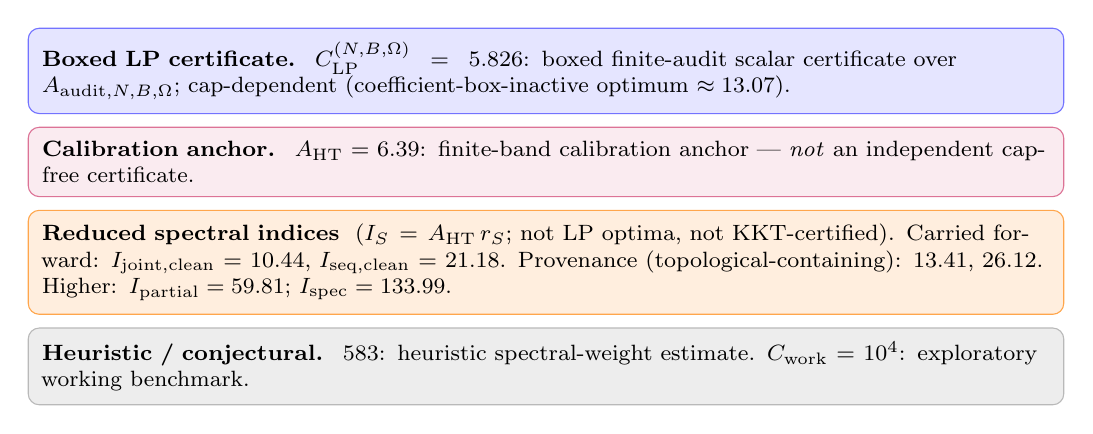
\begin{tikzpicture}[
  cat/.style={draw, rounded corners, align=left, text width=12.8cm, inner sep=5pt, font=\footnotesize},
]
\node[cat, fill=blue!10, draw=blue!55] (l1) {\textbf{Boxed LP certificate.}~ $C_{\mathrm{LP}}^{(N,B,\Omega)}=5.826$: boxed finite-audit scalar certificate over $A_{\mathrm{audit},N,B,\Omega}$; cap-dependent (coefficient-box-inactive optimum $\approx 13.07$).};
\node[cat, fill=purple!8, draw=purple!55, below=1.6mm of l1] (l2) {\textbf{Calibration anchor.}~ $A_{\mathrm{HT}}=6.39$: finite-band calibration anchor --- \emph{not} an independent cap-free certificate.};
\node[cat, fill=orange!13, draw=orange!70, below=1.6mm of l2] (l3) {\textbf{Reduced spectral indices}~ ($I_{S}=A_{\mathrm{HT}}\,r_{S}$; not LP optima, not KKT-certified). Carried forward: $I_{\mathrm{joint,clean}}=10.44$, $I_{\mathrm{seq,clean}}=21.18$. Provenance (topological-containing): $13.41$, $26.12$. Higher: $I_{\mathrm{partial}}=59.81$; $I_{\mathrm{spec}}=133.99$.};
\node[cat, fill=gray!14, draw=gray!55, below=1.6mm of l3] (l4) {\textbf{Heuristic / conjectural.}~ $583$: heuristic spectral-weight estimate. $C_{\mathrm{work}}=10^{4}$: exploratory working benchmark.};
\end{tikzpicture}
\caption{Two-object status of the audited quantities. The entries occupy different mathematical categories and do \emph{not} form one LP/KKT-certified response ladder: only $C_{\mathrm{LP}}=5.826$ is a boxed finite-audit LP/KKT certificate; $A_{\mathrm{HT}}=6.39$ is a calibration anchor (not an independent cap-free certificate); the reduced indices $I_{S}=A_{\mathrm{HT}}\,r_{S}$ are calibrated spectral-norm sensitivity values, not LP optima and not certified; and $583$, $C_{\mathrm{work}}=10^{4}$ are heuristic and exploratory. The topological-containing values $13.41$ and $26.12$ are provenance only.}
\label{fig:ladder}
\end{figure}

%-----------------------------------------------------------
\begin{table}[ht]
\centering
\caption{Anchor sensitivity of the reduced-operator index $I_{S}=A_{\mathrm{HT}}\,r_{S}$. The raw ratios $r_{S}$ are independent of the baseline coefficient box; the absolute calibrated indices inherit the box through the adopted anchor $A_{\mathrm{HT}}=6.39$ (adopted; implied ratio $0.0968$, \S3.2). Values recomputed from the corrected-projector reduced-model output. $^{\dagger}$ box-inactive baseline substituted only as a sensitivity anchor; $^{\ddagger}$ $13.07\times(1+0.0968)$ substituted illustratively --- neither is an independently derived anchor.}
\label{tab:anchor}
\begin{tabular}{lccccc}
\toprule
case & raw $r_{S}$ & $A_{\mathrm{HT}}=6.39$ & $5.826$ & $13.07^{\dagger}$ & $14.33^{\ddagger}$ \\
\midrule
clean joint            & $1.6337$  & $10.44$  & $9.52$   & $21.35$  & $23.42$ \\
clean sequential       & $3.3146$  & $21.18$  & $19.31$  & $43.32$  & $47.51$ \\
sequential provenance  & $4.0874$  & $26.12$  & $23.81$  & $53.42$  & $58.59$ \\
joint provenance       & $2.0993$  & $13.41$  & $12.23$  & $27.44$  & $30.09$ \\
partial                & $9.3607$  & $59.81$  & $54.54$  & $122.34$ & $134.17$ \\
speculative            & $20.9690$ & $133.99$ & $122.17$ & $274.06$ & $300.57$ \\
\bottomrule
\end{tabular}
\end{table}

\section{Matter realisation and compact-object obstruction}\label{sec:matter}
%-----------------------------------------------------------

The selected clean calibrated index is $I_{\mathrm{seq,clean}}\approx21.18$; the earlier $I_{\mathrm{seq,prov}}=26.12$, which depended on the KILL-tainted topological input, is carried only as provenance. This is where the audit turns from optimisation back to physics. A reduced-model index can be selected for conditional scale reconstruction and still fail as a source if the corresponding matter cannot be supported by an equation of state, cannot satisfy the TOV equations, cannot be supplied by any material class, cannot be operated near safely, or has no standards-qualified realisation pathway. This section applies those gates.

\subsection{Illustrative scale mapping for the selected reduced case}

The audit uses an illustrative audit scale mapping (a stated normalisation, not a GR-derived law)
\[
I_{S}\,R^{2}=L_{0}^{2},\qquad L_{0}^{2}=10^{6}\,\mathrm{km}^{2},
\]
which converts a reduced-operator index $I_{S}$ to an aperture $R$. The constant $L_{0}^{2}=10^{6}\,\mathrm{km}^{2}$ is a chosen reference normalisation, not a derived law. Because $M=uc^{2}R/G\propto R$ and the mean density scales as $R^{-2}$ at fixed $u$, the value of this constant sets which matter gate binds: a larger constant gives a larger aperture, larger mass and lower density, a smaller constant the reverse. The convention-independent statement is simply that a $u=0.20$ shell at any macroscopic aperture is an astronomical-mass object; the specific mass and density values below hold under the stated convention.
For the clean sequential index (raw ratio $r_{\mathrm{seq,clean}}=3.3146$, anchor $A_{\mathrm{HT}}=6.39$, so $I_{\mathrm{seq,clean}}=A_{\mathrm{HT}}\,r_{\mathrm{seq,clean}}\simeq21.18$), the mapping gives
\[
R = \sqrt{L_{0}^{2}/I_{\mathrm{seq,clean}}} = \sqrt{10^{6}/21.18} \simeq 217.3\,\mathrm{km}.
\]
This reconstruction is conditional on (i) the reduced projector $Q_{\mathrm{red}}$ and kernel family, (ii) the raw ratio $r_{S}$, (iii) the anchor $A_{\mathrm{HT}}=6.39$, (iv) the scale constant $L_{0}^{2}=10^{6}\,\mathrm{km}^{2}$, (v) the compactness $u=0.20$, and (vi) the selected WarpFactory shell reconstruction. At fixed raw ratio, compactness and $L_{0}$, the outputs scale as
\[
R\propto A_{\mathrm{HT}}^{-1/2},\qquad M\propto A_{\mathrm{HT}}^{-1/2},\qquad \rho\propto A_{\mathrm{HT}},
\]
so $217.3\,\mathrm{km}$, $29.4\,M_{\odot}$ and $3.5\times10^{15}\,\mathrm{kg\,m^{-3}}$ are conditional reconstructions, not convention-independent physical predictions.
The compactness is held fixed at
\[
u=\frac{GM}{c^{2}R}=0.20,
\]
so the mass associated with the retained rung is
\[
M = \frac{u c^{2}R}{G} \simeq 29.4\,M_{\odot}.
\]
The same compactness gives
\[
\frac{r_{s}}{R}=2u=0.40,
\qquad
\frac{v_{\mathrm{esc}}}{c} = \sqrt{2u} = \sqrt{0.4} \simeq 0.6325.
\]
The value $u=0.20$ is used as a scale convention for comparing rungs. It keeps the shell outside the horizon regime, since $r_{s}/R=2u=0.40$, while still placing the source ledger in a relativistic compact-object regime. Holding $u$ fixed prevents the comparison between rungs from mixing response gain with a changing compactness assumption.

Under the stated compactness convention, the outer aperture lies outside the Schwarzschild radius associated with the total mass; this alone does not exclude all trapped surfaces. It is not engineering-scale matter. It is a compact-object-scale source ledger: tens of solar masses inside a characteristic aperture of order $200\,\mathrm{km}$.

The scale $R$ should be read as the characteristic aperture of the source shell surrounding the controlled region. It is not the radius of a spacecraft body, and $M$ is not payload mass. It is the source-ledger mass associated with the shell-scale geometry.

\begin{figure}[ht]
\centering
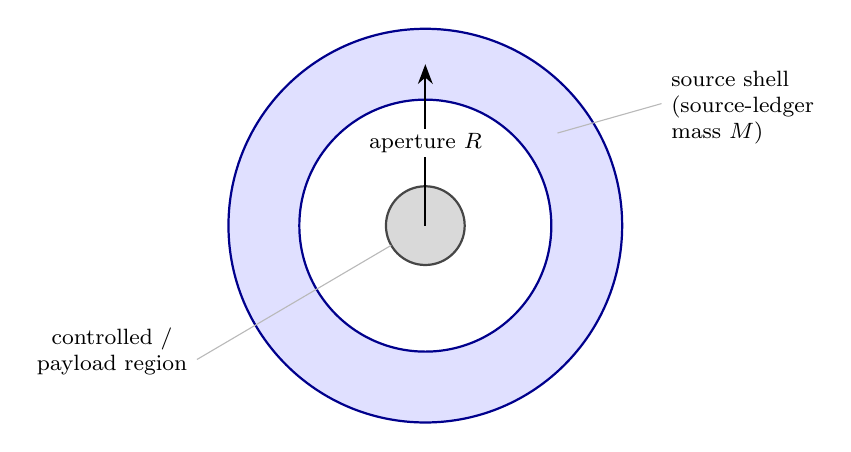
\begin{tikzpicture}[font=\footnotesize, scale=1.0]
  \fill[blue!12, even odd rule] (0,0) circle (2.5) (0,0) circle (1.6);
  \draw[thick, blue!55!black] (0,0) circle (2.5);
  \draw[thick, blue!55!black] (0,0) circle (1.6);
  \fill[gray!30] (0,0) circle (0.5);
  \draw[thick, gray!55!black] (0,0) circle (0.5);
  \draw[-{Stealth[length=2.5mm]}, thick] (0,0) -- (0,2.05);
  \node[fill=white, inner sep=1.5pt] at (0.0,1.05) {aperture $R$};
  \draw[gray!55,thin] (210:0.5) -- (-2.9,-1.7);
  \node[align=center, anchor=east] at (-2.9,-1.6) {controlled /\\payload region};
  \draw[gray!55,thin] (35:2.05) -- (3.0,1.55);
  \node[align=left, anchor=west] at (3.0,1.5) {source shell\\(source-ledger\\mass $M$)};
\end{tikzpicture}
\caption{Source-shell concept (schematic; \emph{not to scale}). The audited scale describes a source shell of characteristic aperture $R$ carrying the source-ledger mass $M$, surrounding a much smaller controlled/payload region. Here $R$ is the aperture of the source shell, not the radius of a spacecraft body, and $M$ is source-ledger mass, not payload mass. This is a conceptual schematic only: it is \emph{not} a spacecraft design and \emph{not} a buildable architecture, and it introduces no dimensions beyond $R$, $M$ and the compactness used in the text.}
\label{fig:source-shell}
\end{figure}

The distinction matters. Horizon safety is a geometric condition. It says the scale ledger does not immediately form a Schwarzschild horizon. It does not say that any material, equation of state, assembly process or operational environment exists for such a source.

\subsection{Ordinary isotropic compact-star EOS/TOV comparison gate}

This gate compares the reconstructed scale against ordinary isotropic compact-star equilibrium; it does \emph{not} solve the equilibrium of the reconstructed hollow shell. The reconstructed geometry is a hollow shell with an inner vacuum region ($R_{1}=R/2$); its equilibrium requires inner-boundary matching or junction conditions, radial and tangential stress treatment, and a separate stability analysis, which are outside the present audit. For the comparison gate, a static isotropic compact source must satisfy the TOV system. Here $\varepsilon(r)$ denotes energy density, so $\varepsilon/c^{2}$ is the corresponding mass density. In the notation used here,
\[
\frac{dP}{dr}
= -\,\frac{
G\bigl(\varepsilon/c^{2}+P/c^{2}\bigr)
\bigl(m+4\pi r^{3}P/c^{2}\bigr)
}{
r^{2}\bigl(1-2Gm/(c^{2}r)\bigr)
},
\qquad
\frac{dm}{dr}
= 4\pi r^{2}\varepsilon/c^{2}.
\]
The boundary conditions are $m(0)=0$, $P(R)=0$, and $M=m(R)$. The question is whether any audited isotropic static equation of state supplies a pressure-density relation $P(\varepsilon)$ for which the solution reaches $M\simeq29.4\,M_{\odot}$ at $R\simeq217.3\,\mathrm{km}$ and $u=0.20$. \cite{Wald1984}

The audit result is negative. The electron-degenerate relativistic polytrope reproduces the familiar white-dwarf calibration~\cite{Chandrasekhar1931}, not the retained rung. The audited isotropic set comprises three meaningful entries --- a $\gamma=2$ nuclear-matter polytrope, the Chandrasekhar white-dwarf polytrope (integrator calibration $M_{\max}=1.44\,M_{\odot}$), and the Rhoades--Ruffini causal upper bound ($M_{\max}\simeq3.2\,M_{\odot}$) --- together with a constant-density Schwarzschild-interior reference (unphysical, $c_{s}=\infty$) and an out-of-scope anisotropic placeholder; the operative leg is the causal bound, whose $\simeq3.2\,M_{\odot}$ ceiling lies far below the required $\simeq29.4\,M_{\odot}$. Canonical neutron-star equations of state compatible with current observational constraints support masses of only a few solar masses at radii of order $10$ to $15\,\mathrm{km}$, not $29.4\,M_{\odot}$ at roughly $217\,\mathrm{km}$. The neutron-star observational programme has also tightened the allowed EOS space: GW170817 constrains the tidal deformability of ordinary neutron stars, while PSR J0740+6620 is a high-mass measured neutron star near $2.08\,M_{\odot}$, still far below the retained-rung mass scale. For ordinary neutron-star matter matched to a known low-density equation of state, causal upper-bound analyses (the Rhoades--Ruffini limit) give maximum masses of only a few solar masses, many factors below the reconstructed scale, so the obstruction is not merely one of catalogue density or horizon safety. \cite{LIGO_GW170817_2017,Fonseca2021J0740,RhoadesRuffini1974}

The failure is not that the retained rung is too close to a horizon. At $u=0.20$, it is not. The failure is that no audited isotropic static EOS closes the TOV system at the required mass-radius pair. Under the illustrative scale mapping, the retained source-scale reconstruction lies far above standard causal neutron-star mass bounds while remaining below the immediate horizon threshold, so the failure is stronger than a catalogue-density mismatch. Anisotropic compact-object matter is a possible future audit direction, but it would need to close a mass-scale gap of many factors while preserving the declared energy-condition, stability and ledger constraints; it is not a solution within the present result.

\subsection{Density and materials gate}

The density obstruction is the simplest numerical way to see the same problem. In the reconstructed retained-rung source, the peak mass density is obtained from
\[
\rho_{\mathrm{peak}} = T_{00}^{\max}/c^{2}.
\]
For the clean retained value $I_{\mathrm{seq,clean}}\approx21.18$, the reconstructed single-shell source at $R\simeq217.3\,\mathrm{km}$ and $u=0.20$ gives
\[
\rho_{\mathrm{peak}} \simeq 3.5\times10^{15}\,\mathrm{kg\,m^{-3}}\quad(\pm\,{\sim}15\%\ \text{grid scatter over }N=24/32/48).
\]
(The earlier $I_{\mathrm{seq,prov}}=26.12$ case, at $R\simeq195.7\,\mathrm{km}$, gives $\rho_{\mathrm{peak}}\simeq4.4\times10^{15}\,\mathrm{kg\,m^{-3}}$.)
Across the audited rungs at fixed compactness, the peak-density scale lies in the $10^{15}$ to $10^{16}\,\mathrm{kg\,m^{-3}}$ range. This is below nuclear density at the retained rung, but it is still compact-object density, not condensed-matter density.

The audited material catalogue contains 36 candidate material classes. It includes ordinary structural materials, dense metallic auxiliaries such as Nb$_{3}$Sn, SRF niobium and REBCO HTS, high-stiffness metamaterial candidates, and ML-generated inorganic-crystal candidates from MatterGen and MatterSim used only as auxiliary candidate-generation tools. None approaches the source-density scale. Such tools can propose condensed-matter candidates for auxiliary roles, but they do not change the density scale: molecular and crystalline matter remain many orders of magnitude below compact-object source density. The densest catalogue entries remain of order $10^{4}\,\mathrm{kg\,m^{-3}}$. \cite{MatterGen2024,MatterSim2024}

The shortfall is therefore
\[
\frac{\rho_{\mathrm{peak}}}{\rho_{\mathrm{catalogue,max}}}
\approx
\frac{10^{15}\,\mathrm{kg\,m^{-3}}}{10^{4}\,\mathrm{kg\,m^{-3}}}
= 10^{11}.
\]
Allowing for the full peak-density range, the gap is a factor of $10^{11}$ to $10^{12}$, or 11 to 12 orders of magnitude. This is not a small optimisation gap inside a materials catalogue. It is the difference between engineered matter and compact-object matter.

\begin{figure}[t]
\centering
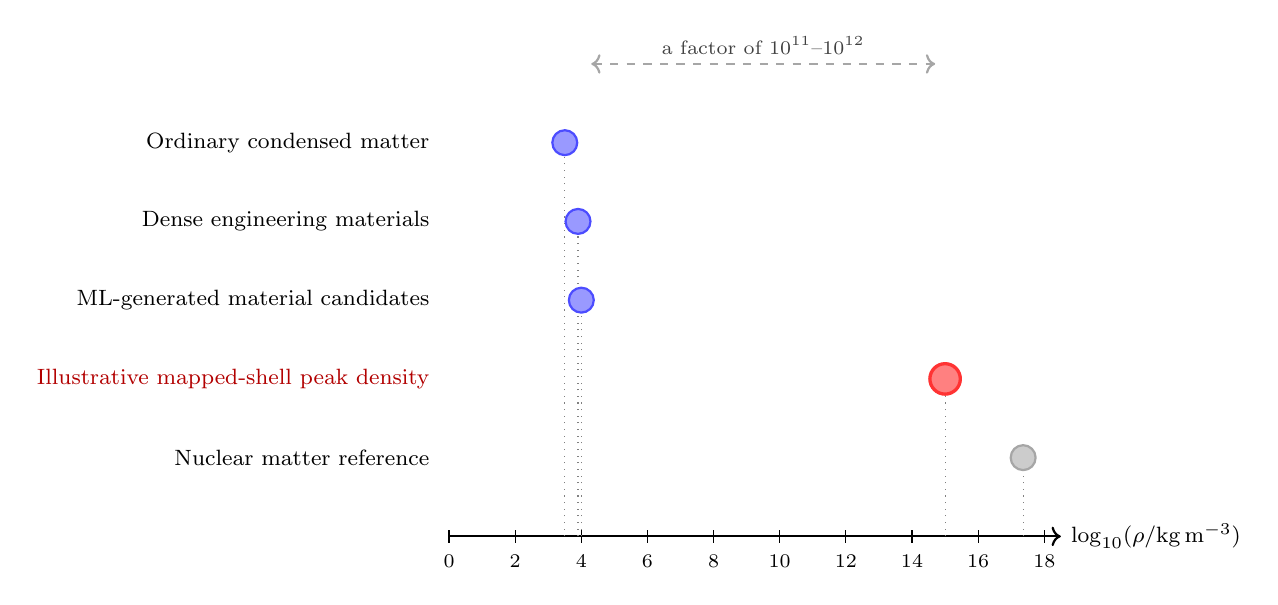
\begin{tikzpicture}[
  every node/.style={font=\small},
  catlabel/.style={font=\footnotesize, anchor=east, align=right},
  ord/.style={circle, draw=blue!70, fill=blue!40, minimum size=9pt, inner sep=0pt, thick},
  src/.style={circle, draw=red!80, fill=red!50, minimum size=11pt, inner sep=0pt, very thick},
  ref/.style={circle, draw=gray!70, fill=gray!40, minimum size=9pt, inner sep=0pt, thick},
  xscale=0.42,
]
\node[catlabel] at (-0.3, 4) {Ordinary condensed matter};
\node[catlabel] at (-0.3, 3) {Dense engineering materials};
\node[catlabel] at (-0.3, 2) {ML-generated material candidates};
\node[catlabel, red!70!black] at (-0.3, 1) {Illustrative mapped-shell peak density};
\node[catlabel] at (-0.3, 0) {Nuclear matter reference};
\draw[->, thick] (0, -1) -- (18.5, -1) node[right, font=\footnotesize]{$\log_{10}(\rho/\mathrm{kg\,m^{-3}})$};
\foreach \x in {0,2,4,6,8,10,12,14,16,18} {
  \draw (\x, -1.08) -- (\x, -0.92);
  \node[below=1pt, font=\scriptsize] at (\x, -1.08) {\x};
}
\foreach \x/\y in {3.5/4, 3.9/3, 4.0/2, 15.0/1, 17.36/0} {
  \draw[dotted, gray] (\x, -1) -- (\x, \y);
}
\node[ord] at (3.5, 4) {};
\node[ord] at (3.9, 3) {};
\node[ord] at (4.0, 2) {};
\node[src] at (15.0, 1) {};
\node[ref] at (17.36, 0) {};
\draw[<->, dashed, gray!70, thick] (4.3, 5.0) -- (14.7, 5.0);
\node[above, font=\scriptsize, gray!50!black, align=center] at (9.5, 5.0)
  {a factor of $10^{11}$--$10^{12}$};
\end{tikzpicture}
\caption{Density-scale obstruction behind the matter-realisation gate. Ordinary condensed matter, dense engineering materials and ML-generated material candidates remain near $10^{3}$ to $10^{4}\,\mathrm{kg\,m^{-3}}$, while the illustrative mapped single-shell reconstruction reaches peak density near $10^{15}\,\mathrm{kg\,m^{-3}}$ under the audit-chain scale convention. The shortfall is a factor of $10^{11}$ to $10^{12}$, or 11 to 12 orders of magnitude. This figure is a scale diagnostic only; closing the density gap would still leave the EOS, TOV, operations and standards gates. The nuclear-matter marker is a reference scale, not a candidate engineering material.}
\label{fig:density-gap}
\end{figure}

The material candidates are still useful, but only in the correct role. They may support structures, control systems, cryogenic hardware, radiators, superconducting auxiliaries or instrumentation. They do not supply the source mass. Treating them as source-matter candidates at $10^{15}$ to $10^{16}\,\mathrm{kg\,m^{-3}}$ would be a category error.

\subsection{Operations and self-gravity gate}

At fixed compactness $u=0.20$, the surface escape-velocity ratio is $v_{\mathrm{esc}}/c\simeq0.6325$. That alone puts the near-source environment outside ordinary spacecraft operations. Station-keeping, proximity navigation, communications and inspection cannot be treated with ordinary low-gravity engineering assumptions near such a potential well.

A simple tidal estimate makes the point. Over a separation $\Delta r$, the differential acceleration near radius $R$ scales as
\[
\Delta a \sim \frac{2GM}{R^{3}}\,\Delta r.
\]
With $M\simeq29.4\,M_{\odot}$ and $R\simeq217.3\,\mathrm{km}$, the differential acceleration is of order $2GM/R^{3}\simeq7.6\times10^{5}\,\mathrm{s^{-2}}$ per metre (about $8\times10^{4}\,g$ per metre); the environment is not an ordinary mission-architecture regime. Lowering the compactness would reduce the operational hazard, but it would also change the surface metric perturbation and the scale ledger. The retained-rung analysis is explicitly at fixed $u=0.20$.

This is independent of the materials gate. Even if a hypothetical matter model closed the density and EOS problems, the resulting object would still demand compact-object operations discipline, not ordinary spacecraft proximity engineering.

\subsection{Standards and qualification gate}

The standards gate is included as engineering context, not as physics. The audited aerospace qualification framework (NASA, ECSS and GSFC documents, supplemented by FMEA and FTA) can qualify auxiliary hardware---support structures, materials and processes, verification, structural and fracture control, environmental and electromagnetic testing---but it contains no qualification pathway for compact-object source matter and does not constitute a source-realisation route. Standards qualify hardware; they neither certify nor exclude the source itself. \cite{NASASP20166105,GSFC7000B,NASASTD6016C,ECSSEST1002C}

\subsection{Independent gate failures}

The gates fail independently. The EOS / TOV gate fails because no audited isotropic static EOS supports the required mass-radius pair. The materials gate fails because no catalogued material approaches the source density. The operations gate fails because the compactness creates a near-source environment outside ordinary station-keeping and proximity assumptions. The standards gate fails because the qualification framework recognises support and auxiliary hardware, not compact-object source matter.

The conclusion is therefore stronger than a single negative test. The clean retained $I_{\mathrm{seq,clean}}\approx21.18$ rung survives the operator-side audit, but every matter-realisation route tested in this paper fails. The correct physical interpretation is not "a buildable source with a large coefficient". It is "a retained reduced-model index whose implied source is not realised by the audited matter, operations or standards gates."

\begin{figure}[t]
\centering
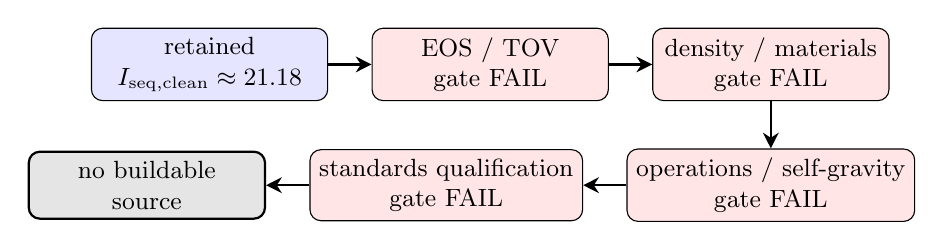
\begin{tikzpicture}[
  every node/.style={font=\small},
  gate/.style={draw, rounded corners, minimum width=3.0cm, minimum height=0.85cm, align=center, fill=red!10},
  start/.style={draw, rounded corners, minimum width=3.0cm, minimum height=0.85cm, align=center, fill=blue!10},
  endbox/.style={draw, rounded corners, minimum width=3.0cm, minimum height=0.85cm, align=center, fill=gray!20, thick},
  arr/.style={-{Stealth[length=2mm,width=2mm]}, thick},
]
\node[start] (start) at (0,0) {retained\\$I_{\mathrm{seq,clean}}\approx21.18$};
\node[gate, right=0.55cm of start] (eos) {EOS / TOV\\gate FAIL};
\node[gate, right=0.55cm of eos] (mat) {density / materials\\gate FAIL};
\node[gate, below=0.6cm of mat] (ops) {operations / self-gravity\\gate FAIL};
\node[gate, left=0.55cm of ops] (std) {standards qualification\\gate FAIL};
\node[endbox, left=0.55cm of std] (nogo) {no buildable\\source};
\draw[arr] (start) -- (eos);
\draw[arr] (eos) -- (mat);
\draw[arr] (mat) -- (ops);
\draw[arr] (ops) -- (std);
\draw[arr] (std) -- (nogo);
\end{tikzpicture}
\caption{Matter-realisation gate structure. The selected clean calibrated reduced index $I_{\mathrm{seq,clean}}\approx21.18$ is passed to independent source-side gates. The EOS/TOV, density/materials, operations/self-gravity and standards-qualification gates fail on separate grounds. The diagram is not a causal sequence; failure of any one gate would be sufficient to block source realisation.}
\label{fig:gate-chain}
\end{figure}

%-----------------------------------------------------------
\section{Geometry verification and scope}\label{sec:verification}
%-----------------------------------------------------------

The operator-side and matter-side results answer different questions. Section 3 computes the boxed finite scalar certificate $C_{\mathrm{LP}}^{(N,B,\Omega)}$; Section 4 computes reduced spectral ratios $r_{S}$ and calibrated indices $I_{S}$. Neither directly evaluates the continuum target $C[T]$, and equivalence between the two finite constructions has not been proved. Section 5 asks whether the selected clean calibrated index corresponds to any source that can be realised as matter. There is a third, narrower check: whether the metric and stress-energy reconstruction used for the scale ledger is algebraically consistent as a geometry. That is the role of the WarpFactory verification.

For each selected case (the calibration anchor $A_{\mathrm{HT}}=6.39$ and the reduced indices $I_{\mathrm{joint,clean}}=10.44$, $I_{\mathrm{joint,prov}}=13.41$, $I_{\mathrm{seq,clean}}=21.18$, $I_{\mathrm{seq,prov}}=26.12$, $I_{\mathrm{partial}}=59.81$, $I_{\mathrm{spec}}=133.99$), the audit reconstructs the corresponding Bobrick--Martire passive single-shell geometry at fixed compactness $u=0.20$ and at the implied $(R,M)$ scale. The WarpFactory \texttt{verifyTensor} pipeline then checks the metric, Einstein tensor and reconstructed stress-energy tensor for tensor-algebra consistency. All seven cases return
\[
\texttt{verifyTensor}=\texttt{PASS}.
\]
The cases are the calibration anchor $A_{\mathrm{HT}}=6.39$ at $R\simeq395.6\,\mathrm{km}$, the clean joint $I_{\mathrm{joint,clean}}\approx10.44$ at $R\simeq309.5\,\mathrm{km}$, $I_{\mathrm{joint,prov}}=13.41$ at $R\simeq273.0\,\mathrm{km}$, the clean retained $I_{\mathrm{seq,clean}}\approx21.18$ at $R\simeq217.3\,\mathrm{km}$, $I_{\mathrm{seq,prov}}=26.12$ at $R\simeq195.7\,\mathrm{km}$, $I_{\mathrm{partial}}=59.81$ at $R\simeq129.3\,\mathrm{km}$, and $I_{\mathrm{spec}}=133.99$ at $R\simeq86.4\,\mathrm{km}$. \cite{WarpFactory2024,WarpFactoryCQG2024,WarpFactoryRepo}

The clean rungs $I_{\mathrm{joint,clean}}\approx10.44$ ($R\simeq309.5\,\mathrm{km}$) and $I_{\mathrm{seq,clean}}\approx21.18$ ($R\simeq217.3\,\mathrm{km}$) were each reconstructed as their own single-shell geometries at $u=0.20$ and checked directly: \texttt{verifyTensor}$=$\texttt{PASS} for both, with the same dimensionless metric depth $h_{tt}^{\max}\simeq0.50$ as the other fixed-compactness cases. They are part of the verified set; the topological-containing values $13.41$ and $26.12$ are preserved as provenance.

This check is deliberately narrow. It is an implementation-consistency test (metric-only input; the stress-energy is derived from the metric via $G/8\pi G$, not supplied independently): it verifies that the reconstructed geometry is internally consistent at the metric, Einstein-tensor and stress-energy level. Section~3 computes the boxed finite-audit certificate $C_{\mathrm{LP}}$; Section~4 computes reduced spectral ratios $r_{S}$ and calibrated indices $I_{S}$. Neither section evaluates the continuum target $C[T]$, and WarpFactory computes none of $C[T]$, $C_{\mathrm{LP}}$, $r_{S}$ or $I_{S}$. The WarpFactory check does not close the EOS or TOV equations, identify material source matter, or validate any propulsion or device claim. The geometry check and the response audit are complementary, not interchangeable.

The same separation of roles applies to the auxiliary material and standards work. A support structure, superconducting auxiliary, control system, catalogue material or standards-qualified component may be real engineering while still not being the source matter required by the stress-energy tensor. The article therefore keeps three layers separate: geometry consistency, operator-side response certification, and matter-realisation viability. Passing one layer does not imply passing the others.

The clean retained value $I_{\mathrm{seq,clean}}\approx21.18$ is not a speed and is not a propulsion performance. Informal pattern-speed comparisons---identifying the dimensionless coefficient $C$ with an effective velocity, as in parts of the warp-drive literature---lie outside the proof chain of this paper and are not used in any result.

The scope of the negative result is therefore unchanged by any such comparison. The paper does not claim a universal no-go theorem for every conceivable warp-shell programme. It claims a boxed finite-audit LP certificate, a reduced spectral sensitivity study and a matter-realisation failure for the explicitly defined admissible class $A_{+}$, the audited stationary positive-energy background, the matched-control suite and the finite-band campaign described above. Branches outside $A_{+}$, including non-passive response, modified gravity, macroscopic energy-condition violation or fully dynamical three-dimensional numerical-relativity configurations, are outside the result rather than refuted by it.

%-----------------------------------------------------------
\section{Discussion}\label{sec:discussion}
%-----------------------------------------------------------

The paper has two linked conclusions. The first is operator-side: within the audited admissible class $A_{+}$, the selected clean calibrated index is $I_{\mathrm{seq,clean}}\approx21.18$ (the earlier $I_{\mathrm{seq,prov}}=26.12$, which depended on the KILL-tainted topological input, is carried as provenance), while the exploratory working benchmark remains $C_{\mathrm{work}}=10^{4}$. The second is matter-side: the selected clean calibrated index implies a compact-object-scale source, and every matter-realisation gate tested in §5 fails. These conclusions are linked but not identical. The operator-side result can be sharpened without solving the matter problem; conversely, a new matter model would not by itself change the operator-side certificate.

The cleanest way to read the result is therefore as a map of bottlenecks. It does not say that every conceivable warp-shell programme is impossible. It says that the audited positive-energy, stationary, passive-response, matched-control-orthogonal source class has a retained reduced-model index and no realised matter source in the tested catalogue. That is narrower than a universal no-go theorem, but stronger than a numerical example: the result identifies which mathematical, computational and matter-side gates would have to change before the conclusion could change.

The framework contains one boxed LP/KKT certificate and a separate calibrated reduced spectral sensitivity model; it is not a single certified response ladder. The LP/KKT certificate (for $C_{\mathrm{LP}}$) is tied to the constructed finite audit operator, matched-control projector, coefficient box and discretisation stated above. It should not be read as a continuum theorem for all positive-energy warp-shell geometries, nor as a fully GR-derived linearised-Einstein response bound. Its role is methodological and diagnostic: it supplies a reproducible stress-energy-first audit protocol linking operator certificates to source-scale reconstruction and matter-realisation gates. A fully physical extension would derive the source-to-geometry operator from the linearised Einstein constraint system on the chosen warp-shell background, prove the matched-control projection, quantify truncation and polyhedron-approximation errors, and reduce or remove calibration choices. That extension is the natural next stage for a source-realisation audit workbench.

This study contains two linked but mathematically distinct computations. The first is a boxed, $2880$-dimensional LP/KKT certificate for one scalar matched-control-orthogonal observable on a finite sampled admissible class. The second is a $32$-dimensional reduced spectral model that measures singular-value ratios under controlled operator compositions and converts them to calibrated indices through $A_{\mathrm{HT}}=6.39$. Equivalence between these two constructions has not been proved. Their value lies in their complementary audit roles: the first tests finite constrained optimisation and dual certification; the second tests reduced-model sensitivity to operator modifications. A fully physical source-realisation workbench must derive the source-to-geometry operator and matched-control projector from the linearised Einstein constraints, connect reduced and full-order models, implement observer-robust energy-condition testing, quantify truncation and polyhedron errors, analyse hollow or anisotropic shell equilibrium, and eliminate arbitrary calibration and scale mappings where possible. An attempted mechanism-level comparison between the reduced spectral ratio and the full boxed-LP certificate could not be established from the frozen artefacts: the reduced Gaussian kernel and the full \texttt{delta\_H} LP objective are not generated by a common documented source-to-response operator, so the additive reduced-kernel perturbation has no derived full-order counterpart. The numerical surrogate lift was therefore classified as \emph{mapping not established} and is not used as evidence of predictive equivalence. Deriving a common full-order operator is a defined work package for the proposed source-realisation workbench.

The first bottleneck is sharpening the working envelope toward a proved bound. The passive spectral-weight estimate suggests $C_{\mathrm{passive}}=583$, but the paper retains $C_{\mathrm{work}}=10^{4}$ because three theorem gaps remain open. Closing the small-denominator extension $Q3a$ would extend the dual certificate from the audited stationary background to a wider family of stationary admissible backgrounds. Deriving the sharp passive sum-rule coefficient $Q3d$ would determine whether the heuristic spectral-weight estimate could be promoted to a certified bound. Controlling the finite-band dispersion trade-off $Q3e$ would show whether the finite-band spectral result $U\leq6.39$ is stable under bandwidth changes. These are mathematical sharpening tasks. None would by itself create a buildable source.

The second bottleneck is operator-side validation above the retained rung. The value $I_{\mathrm{partial}}=59.81$ is not retained because two Tier-2 mechanism factors are still estimate-only. Upgrading it would require direct audit-chain validation of the multipole tensor-spherical-harmonic basis-completion factor and the matched-control-equivalent coupling factor, including primal LP tests and ledger reconciliation. The value $I_{\mathrm{spec}}=133.99$ is more remote. It depends on a regularised extremiser candidate with a provenance gap and a singular-or-unstable risk. Upgrading that rung would require an honest support-energy ledger and a stability check strong enough to remove those flags. Until then, the larger values remain informative about relaxed optimisation, not certified outcomes.

The third bottleneck is matter realisation. The isotropic static EOS/TOV gate fails at the retained mass-radius pair, but this does not exhaust all mathematical possibilities. A controlled anisotropic-pressure model, a rotating compact configuration, or a genuinely new compact-object equation of state could in principle be tested against the same scale ledger. Such a model would need to solve the relevant equilibrium equations, preserve the energy conditions required by $A_{+}$, avoid ghost or tachyonic constitutive modes, and maintain the full energy ledger. Merely raising the density is not enough. A source that reaches $10^{15}\,\mathrm{kg\,m^{-3}}$ but fails EOS closure, stability or conservation would not change the conclusion.

The fourth bottleneck is reproducibility. The calculation combines the boxed LP/KKT certificate, finite-band spectral bounds, passive spectral-weight arguments, operator-composition audits, WarpFactory tensor checks, density reconstruction, material catalogues and standards screening. Each component is individually meaningful, but the scientific value lies in making the chain reproducible end to end. A useful next stage is therefore a source-realisation workbench: one pipeline that takes a candidate source class, constructs the admissibility polyhedron, computes the projected response coefficient, records the primal and dual certificates, reconstructs the geometry, evaluates the density and compactness ledger, and applies the matter and standards gates. Such a workbench would not assume success. Its purpose would be to make failure modes explicit and repeatable.

The final bottleneck is interpretation. Operator-side improvements should not be described as propulsion progress unless the matter side also moves. Auxiliary materials, superconducting components, control hardware and standards-qualified subsystems may be useful engineering artefacts, but they do not constitute source matter at compact-object density. Likewise, geometry verification confirms tensor-algebra consistency, not buildability. The paper’s future path is therefore not to seek a larger number alone. It is to reduce the gap between response certification and source realisation, while preserving the separation between geometry, operator response and matter physics established above.

The next stage is to turn this one-off audit into a reproducible source-realisation workbench: a software pipeline that imports or derives candidate source-to-geometry operators, constructs admissibility polyhedra, computes LP/KKT certificates, verifies reconstructed geometries, applies EOS/TOV and material-density gates, and records provenance so that exotic spacetime claims can be tested rather than merely asserted.

\subsection{Baseline constrained reduction: a feasible reduced-order surrogate}\label{sec:baseline-reduction}
The two-object separation can be probed constructively without asserting equivalence. We tested whether a systematically constructed reduced-order model (ROM) of the boxed audit LP reproduces the full certificate $C_{\mathrm{LP}}=5.826$ \emph{without ever using the optimum}. We generated $160$ feasible snapshots as perturbed-objective optima of the full $2880$-variable boxed LP (interior point; each feasible to $\lVert A_{\mathrm{eq}}\tau\rVert_{\infty}\sim10^{-14}$), deliberately excluding the frozen optimum $\tau_{0}$ from the training set (held-out evaluation only). The snapshot matrix has full numerical rank $160$, so proper-orthogonal-decomposition (POD) bases at $r=16,32,64,128$ and a greedy maximum-residual adaptive basis are all well posed.

Each reduced constrained LP is solved to machine-precision optimality --- duality gap and complementary slackness $\lesssim10^{-13}$, stationarity $\lesssim10^{-14}$, inequality and bound multipliers satisfying their non-negativity conditions (equality multipliers unrestricted), primal feasibility $\lesssim10^{-11}$ --- and, being a restriction of the full feasible set, returns a rigorous lower bound $C_{\mathrm{LP}}^{\mathrm{red}}\le C_{\mathrm{LP}}$. The POD reduction gives $C_{\mathrm{LP}}^{\mathrm{red}}=5.532,\,5.541,\,5.553,\,5.577$ at $r=16,32,64,128$ (relative error $5.04\%\rightarrow4.28\%$); the greedy basis reaches $5.617$ ($3.58\%$) at $r=64$. Over the tested dimensions $r=16,32,64,128$ the relative error decreases only from $5.04\%$ to $4.28\%$, so the tested POD sequence does not provide rapid convergence: the held-out reconstruction error of $\tau_{0}$ in the POD-$64$ span is $65\%$, i.e.\ $\tau_{0}$ is poorly represented by the POD-$64$ span, and the few-per-cent gap persists for both tested basis constructions (the POD and greedy subspaces differ by principal angles up to $89.7^{\circ}$). An independent MATLAB R2026a check (native SVD and \texttt{linprog} dual-simplex) reproduces the rank, the full singular spectrum (agreement $<10^{-13}$), the POD subspace (principal angles $<10^{-3}$~deg) and every reduced $C_{\mathrm{LP}}^{\mathrm{red}}$ to six figures.

We record this as a corroborative order-reduction result: the boxed certificate admits a feasible reduced surrogate accurate to a few percent \emph{as a lower bound}, not a high-accuracy replacement, and the exercise establishes no predictive equivalence between the reduced spectral index and the full certificate. The separate attempt to map the reduced finite-amplitude mechanism onto the full certificate remains \emph{mapping not established}; deriving a common full-order source-to-response operator is a defined task for the proposed workbench.

%-----------------------------------------------------------
\section{Conclusion}\label{sec:conclusion}
%-----------------------------------------------------------

This paper has treated the warp-shell problem from the stress-energy side. Rather than beginning with a desired trajectory or device, it fixed an admissible positive-energy source class $A_{+}$, defined the projected response coefficient $C[T]$, and asked what the audited source and operator families can actually support.

The fixed-operator calculation gives $C_{\mathrm{LP}}=5.826$ and the calibrated finite-band anchor is $A_{\mathrm{HT}}=6.39$. The passive spectral-weight analysis suggests a heuristic estimate $C_{\mathrm{passive}}=583$ (not a proved bound), while the exploratory working benchmark remains $C_{\mathrm{work}}=10^{4}$ until the small-denominator, passive-coefficient and finite-band-dispersion gaps are closed.

Allowing controlled operator-side variation raises the reduced-operator index. The joint reduced-operator composition gives the provenance rung $I_{\mathrm{joint,prov}}=13.41$, and the sequential reduced-operator composition gives $I_{\mathrm{seq,prov}}=26.12$; after removing the KILL-tainted topological input, the clean retained value carried forward is $I_{\mathrm{seq,clean}}\approx21.18$. The higher candidates $I_{\mathrm{partial}}=59.81$ and $I_{\mathrm{spec}}=133.99$ are recorded because they are informative, but they are not retained: the first is partial and the second is speculative. The central operator-side result is therefore not the largest number in the audit, but the largest reduced-operator index that survives the stated model-status discipline. It is a calibrated spectral-norm sensitivity value, not an LP/KKT-certified bound.

The matter-side conclusion is negative. At the clean retained rung, the illustrative scale mapping $I_{S}R^{2}=10^{6}\,\mathrm{km}^{2}$ gives a conditional reconstruction $R\simeq217.3\,\mathrm{km}$. At fixed compactness $u=0.20$, this corresponds to $M\simeq29.4\,M_{\odot}$, $v_{\mathrm{esc}}/c\simeq0.6325$, and a reconstructed peak density $\rho_{\mathrm{peak}}\simeq3.5\times10^{15}\,\mathrm{kg\,m^{-3}}$. The audited isotropic EOS/TOV gate does not close at this mass-radius pair. The materials catalogue remains 11 to 12 orders of magnitude below the required density. The operations and standards gates fail independently. The hollow or anisotropic shell equilibrium problem is not solved here, so this is a comparison-gate failure for ordinary isotropic compact-star sequences, not a universal EOS/TOV no-go for every possible shell stress tensor. Thus the retained reduced-operator index is not a realised source.

The WarpFactory checks add an important but limited consistency test. They confirm tensor-algebra consistency for the reconstructed single-shell geometries at the audited rungs. They do not certify the boxed LP/KKT response coefficient $C_{\mathrm{LP}}$ and do not compute the reduced spectral index $r_{S}/I_{S}$ (WarpFactory computes neither object); they do not supply an equation of state, do not identify material source matter, and do not imply a propulsion device.

The result is therefore neither a buildable warp-drive design nor a universal no-go theorem. It is a finite-audit demonstration: within the explicitly defined positive-energy, stationary, passive-response, matched-control-orthogonal framework, it contains one boxed LP/KKT certificate for a finite scalar observable and a separate calibrated reduced spectral sensitivity study whose selected clean index $I_{\mathrm{seq,clean}}\approx21.18$ is not certified and not a physical response coefficient, and the corresponding matter realisation fails. Changing that conclusion would require changing one of the named gates, not merely quoting a larger relaxed optimisation value.

\section*{Acknowledgements}

The author thanks The London Library for the quiet of its reading rooms and for access to printing facilities during drafting and revision.

\appendix

%-----------------------------------------------------------
\section{Notation and conventions}\label{app:notation}
%-----------------------------------------------------------

The paper uses geometrised-relativistic notation where needed, but keeps the response coefficient dimensionless. The spacetime metric is $g_{\mu\nu}$, the Einstein tensor is $G_{\mu\nu}$, and the stress-energy tensor is $T_{\mu\nu}$. The energy density measured in the source frame is written as $T_{00}$, with mass density $\rho=T_{00}/c^{2}$.

The admissible positive-energy source class is denoted by $A_{+}$. It includes conservation, energy conditions, ledger, no-horizon and constitutive-stability requirements as continuum goals; the finite LP implements only the conservation, moment-closure, sampled stress-cone surrogate and density-cap subset (Appendix~\ref{app:provenance}). The projected response coefficient is $C[T]$. Its source-side normalisation is
\[
C[T] = \frac{c^{4}R}{G\,E_{\mathrm{total}}[T]}\,\bigl\| Q K T \bigr\|_{W}.
\]
Here $K$ is the response operator, $Q$ is the projection away from the matched-control directions, and $W$ defines the weighted norm used in the response audit. The fixed-operator supremum over the admissible class is
\[
C_{\mathrm{max}} = \sup_{T\in A_{+}}C[T].
\]

The main numerical response levels are distinguished by certification status. $C_{\mathrm{LP}}=5.826$ denotes the fixed-operator LP/KKT baseline. $A_{\mathrm{HT}}=6.39$ denotes the calibrated finite-band anchor (numerically equal to the spectral bound $U_{\mathrm{FB}}$ by shared calibration; not an independent LP/KKT certificate). $C_{\mathrm{passive}}=583$ is a heuristic passive spectral-weight estimate, not a proved bound and not a retained ladder rung. $C_{\mathrm{work}}=10^{4}$ is the exploratory working benchmark. The changed-operator values $13.41$ and $26.12$ are original composition outputs (a joint composition and a sequential branch) preserved as provenance, because both include the KILL-tainted topological input; after removing it, the clean operator-side values carried forward are the clean joint $I_{\mathrm{joint,clean}}\approx10.44$ and the clean retained $I_{\mathrm{seq,clean}}\approx21.18$. The values $59.81$ and $133.99$ are recorded but not retained, because their certification statuses are respectively partial and speculative.

The scale convention used throughout the matter-realisation analysis (a stated normalisation, not a relation derived from $C$ alone) is
\[
I_{S}R^{2}=10^{6}\,\mathrm{km}^{2}.
\]
The compactness parameter is
\[
u=\frac{GM}{c^{2}R}.
\]
For the clean retained value $I_{\mathrm{seq,clean}}\approx21.18$, the paper holds $u=0.20$, giving $R\simeq217.3\,\mathrm{km}$, $M\simeq29.4\,M_{\odot}$, and $v_{\mathrm{esc}}/c=\sqrt{2u}\simeq0.6325$. The earlier $I_{\mathrm{seq,prov}}=26.12$ ($R\simeq195.7\,\mathrm{km}$, $M\simeq26.5\,M_{\odot}$) is preserved as provenance.

The terms retained, partial and speculative are used in a restricted audit sense. Retained means that the value survives the currently available certification discipline. Partial means that one or more input factors remain estimate-only. Speculative means that the rung depends on an unresolved provenance or stability problem. These labels do not describe engineering readiness.

The term WarpFactory verification refers only to an implementation-consistency (tensor-algebra) check applied to reconstructed geometries: the metric is the sole input and the stress-energy is derived from it, not supplied independently. A \texttt{verifyTensor} pass confirms consistency of the metric, Einstein tensor and reconstructed stress-energy tensor. It does not certify $C[T]$, solve an EOS/TOV problem, identify source matter or imply a device.



%-----------------------------------------------------------
\section{Provenance and reproducibility}\label{app:provenance}
%-----------------------------------------------------------

This appendix records how the numerical claims in the paper are meant to be audited. It is not a second derivation of the article. Its purpose is to identify which quantities are certificate-level outputs, which are identified ceilings, which are retained operator-side rungs, which are partial or speculative candidates, and which checks are geometry-only.

The calculation used for the present draft is frozen in the author workflow. The frozen inputs include the article source, bibliography, numerical-anchor provenance note, raw extraction log, source-file index and summary note. The working article is built from those frozen inputs through the section-by-section insertion logs. Each inserted section has a saved author-supplied draft, a review file, an insertion log, a compiled PDF checkpoint and page proofs. This gives a reproducibility trail from author prose to rendered article.

The fixed-operator baseline is the most direct certificate. The LP is solved on the audited discretisation with $N=2880$ dimensionless coefficients $\tau_{i}$ and $N_{r}=32$, with $128$ equality constraints, $23809$ inequality constraints and box bounds $\tau_{i}\in[-1.5,1.5]$. The equality block is $A_{\mathrm{eq}}=4N_{r}=128$ conservation rows with $b_{\mathrm{eq}}=0$; the inequality rows are sampled on $N_{\mathrm{cells}}=N_{r}\times12=384$ evaluation cells (radial nodes $\times$ $12$ Fibonacci directions), decomposing as positivity $384$ + density cap $384$ + NEC-surrogate $12\times384=4608$ + WEC-surrogate($\pm$) $24\times384=9216$ + DEC-surrogate(upper/lower) $24\times384=9216$ + one energy-budget row $=23809$; every row regenerates from the frozen basis to machine precision. The recorded tolerance is $10^{-9}$. The box is active at the optimum, so the certificate is that of the bounded-variable programme; its bounded-KKT primal and dual objectives close to machine precision (true gap $\simeq2.06\times10^{-13}$, recorded in the bounded-KKT sidecar), giving
\[
C_{\mathrm{LP}} = 5.826049575311591 \approx 5.826.
\]
This is the fixed-operator LP/KKT certificate for the boxed coefficient class: the box $B=1.5$ is active and is a numerical scaling cap, distinct from the physical density cap, so $5.826$ is the optimum of that boxed class, not the coefficient-box-inactive optimum ($\approx13.07$), and not an extrapolated material result. This certificate was independently corroborated with MATLAB R2026a \texttt{linprog} (interior-point algorithm, exit flag $1$, feasibility residuals $\sim10^{-6}$) on the same frozen $2880$-variable programme, giving $C_{\mathrm{LP}}=5.825968$ (absolute difference $8.16\times10^{-5}$, relative difference $1.4\times10^{-5}$) --- an independent cross-solver corroboration to about five significant figures under the stated MATLAB tolerances, \emph{not} a second machine-precision KKT certificate; the primary certified value remains the HiGHS bounded-variable KKT result. The reduced-order model, the snapshot singular spectrum and the two clean WarpFactory geometry cases were re-verified in the same MATLAB session (bundle \texttt{bridge\_validation\_v14/code\_matlab/consolidated\_reverify/}).

The high-truncation finite-band result is separately recorded. The anchor $A_{\mathrm{HT}}=6.39$ is adopted (hardcoded \texttt{C\_HT}); the gain factor is the \emph{implied} ratio
\[
G_{\mathrm{HT,max}} = A_{\mathrm{HT}}/C_{\mathrm{LP}}-1 \simeq 0.0968,
\]
so that $A_{\mathrm{HT}} = C_{\mathrm{LP}}(1+G_{\mathrm{HT,max}}) \approx 6.39$ is a consistency restatement, not the derivation.
The finite-band upper-bound check records $U\leq6.39<100$. Consistent with the main text, $6.39$ is a calibrated finite-band rung tied to the stated finite construction, not an independent cap-free certificate.

The passive spectral-weight value has a different status. The passivity and spectral-weight calculation identifies
\[
C_{\mathrm{passive}} = 5.826\times100 \approx 583.
\]
This is recorded as a heuristic passive spectral-weight estimate, not a proved bound, not a retained ladder rung and not the working-envelope bound used for the final statement. The article keeps the exploratory working benchmark
\[
C_{\mathrm{work}}=10^{4}
\]
because the small-denominator extension $Q3a$, the sharp passive sum-rule coefficient $Q3d$, and the finite-band dispersion trade-off $Q3e$ remain open.

The changed-operator sensitivity sequence is derived from separate operator-composition audits. The original joint reduced-operator composition output is
\[
I_{\mathrm{joint,prov}} = 13.41479471679897 \approx 13.41,
\]
preserved as provenance; removing the topological factor it contains gives the clean joint $I_{\mathrm{joint,clean}}\approx10.44$.
The sequential reduced-operator composition gives
\[
I_{\mathrm{seq,prov}} = 26.11858079384958 \approx 26.12.
\]
Removing the topological factor (whose mechanism carries an adversarial KILL verdict) and re-running the same composition gives the clean retained value $I_{\mathrm{seq,clean}}\approx21.18$, which is the value carried forward; $26.12$ is preserved here as provenance.
The higher candidate rungs are retained in the audit archive but not in the carried-forward reduced-model hierarchy. The value
\[
I_{\mathrm{partial}}=59.81466502980856 \approx 59.81
\]
is partial because it depends on Tier-2 estimate-only inputs. The value
\[
I_{\mathrm{spec}}=133.99192191862943 \approx 133.99
\]
is speculative because it depends on a regularised extremiser candidate with unresolved provenance and stability flags. These labels are part of the reproducibility record. They are not stylistic qualifiers.

The matter-side numbers are obtained from the retained rung and the fixed compactness convention. The scale convention (a stated normalisation, not a relation derived from $C$ alone) is
\[
I_{S}R^{2}=10^{6}\,\mathrm{km}^{2}.
\]
For the clean retained value $I_{\mathrm{seq,clean}}\approx21.18$, this gives $R\simeq217.3\,\mathrm{km}$. With $u=0.20$,
\[
M=\frac{u c^{2}R}{G} \simeq 29.4\,M_{\odot},
\qquad
\frac{v_{\mathrm{esc}}}{c}=\sqrt{2u}\simeq0.6325.
\]
The clean retained value $I_{\mathrm{seq,clean}}\approx21.18$ was reconstructed at $R\simeq217.3\,\mathrm{km}$ and $u=0.20$, giving \texttt{verifyTensor}$=$\texttt{PASS} and reconstructed peak density
\[
\rho_{\mathrm{peak}} \simeq 3.5\times10^{15}\,\mathrm{kg\,m^{-3}}\quad(\pm\,{\sim}15\%\ \text{grid scatter over }N=24/32/48).
\]
The earlier $I_{\mathrm{seq,prov}}=26.12$ case (preserved as provenance) gives $R\simeq195.7\,\mathrm{km}$, $M\simeq26.5\,M_{\odot}$ and $\rho_{\mathrm{peak}}\simeq4.4\times10^{15}\,\mathrm{kg\,m^{-3}}$.
Across the audited rungs at fixed compactness, the peak-density scale lies in the $10^{15}$ to $10^{16}\,\mathrm{kg\,m^{-3}}$ range. The material catalogue remains approximately 11 to 12 orders of magnitude below that range.

The WarpFactory checks are recorded separately because they test a different question. For the seven reconstructed single-shell geometries corresponding to the calibration anchor $A_{\mathrm{HT}}=6.39$ and the reduced indices $I_{\mathrm{joint,clean}}=10.44$, $I_{\mathrm{joint,prov}}=13.41$, $I_{\mathrm{seq,clean}}=21.18$, $I_{\mathrm{seq,prov}}=26.12$, $I_{\mathrm{partial}}=59.81$ and $I_{\mathrm{spec}}=133.99$, the \texttt{verifyTensor} check returns PASS~\cite{WarpFactoryCQG2024}. The clean rungs $I_{\mathrm{joint,clean}}\approx10.44$ and $I_{\mathrm{seq,clean}}\approx21.18$ were verified on MATLAB R2026a (CPU, \texttt{tryGPU}$=0$; 2026-06-19), with $h_{tt}^{\max}\simeq0.50$ consistent with the fixed-compactness family. This verifies tensor-algebra consistency of the metric, Einstein tensor and reconstructed stress-energy tensor. It does not certify the response coefficient, the EOS/TOV closure, the material catalogue, operational feasibility or a device claim.

The figures in the paper are generated from the same provenance chain. Figure 1 is a schematic of the stress-energy-first audit flow. Figure 2 summarises the response hierarchy and its certification statuses. Figure 3 is a schematic of the source-shell structure surrounding the controlled region. Figure 4 displays the density-scale obstruction. Figure 5 displays the independent matter-realisation gates. The figures are explanatory summaries of the audited quantities; they are not independent sources of numerical evidence.

The reproducibility artefact set provided in the companion review archive comprises: the raw LP matrices $A_{\mathrm{eq}}$, $b_{\mathrm{eq}}$, $A_{\mathrm{ineq}}$, $b_{\mathrm{ineq}}$ and objective vector $\ell$; the primal solution $\tau$, the dual variables $(\lambda,\mu)$ and the box reduced costs $(\alpha,\beta)$ with bounded-KKT residuals (recorded with the box cap-sensitivity table in the bounded-KKT sidecar certificate); the explicit construction code for $K$, $Q$, $W$ and the mechanism operators $K_S$ (Appendix~\ref{app:operators}); the HiGHS solver logs; and the WarpFactory reconstruction and \texttt{verifyTensor} scripts for the audited shells. Providing these turns the certificate-level statements from reported solver outputs into independently checkable computations.

The reproducibility limits are as important as the reproduced values. The audit establishes the stated certificates on the stated discretisations, operator families and admissibility class. It does not prove that every possible positive-energy warp-shell construction fails. It does not close the open theorem gaps. It does not validate the partial or speculative rungs. It does not turn auxiliary material candidates into source matter. It does not turn a geometry check into a propulsion result. Those limits are part of the result because they define what an independent reproduction should and should not be expected to confirm.

\section{Operator definitions for the finite audit}\label{app:operators}

This appendix records the explicit finite-dimensional operators used in Sections 3 and 4, so that the LP/KKT results are reproducible rather than merely reported. The reduced spectral operators act on the $N_{r}=32$ radial grid, a radial coefficient vector $x\in\mathbb{R}^{N_{r}}$ on nodes $z_{i}=(i-1)/(N_{r}-1)$. The full LP projector $Q_{\mathrm{LP}}$ and objective $\ell$ act in the $N=2880$ coefficient space (radial resolution $N_{r}=32$, ten stress components, nine low multipoles).

\emph{Response operator $K$.} A causal lower-triangular kernel,
\[
K_{ij}=\exp\!\bigl(-(z_{i}-z_{j})^{2}/\sigma^{2}\bigr)\ \ (i\ge j),\qquad K_{ij}=0\ \ (i<j),\qquad \sigma=0.10 .
\]

\emph{Full baseline matched-control projector $Q_{\mathrm{LP}}$.} The boxed finite-audit LP of Section~\ref{sec:fixed-op} uses $Q_{\mathrm{LP}}=I-P_{\mathrm{LP}}$ acting on the full $N=2880$-dimensional coefficient space, where $P_{\mathrm{LP}}$ is the orthogonal projector (built by \texttt{np.linalg.qr} of the control matrix) onto the span of ten physically motivated matched-control templates: uniform, gradient and quadrupole density channels, and isotropic, loop and directional stress channels. It enters the LP objective through the matched-control-orthogonalised response vector $\ell$ of the \texttt{delta\_H} observable, and the KKT certificate is stated over $A_{\mathrm{audit},N,B,\Omega}$. This full projector is a \emph{different} operator from the reduced $Q_{\mathrm{red}}$ below --- different space ($\mathbb{R}^{2880}$ vs $\mathbb{R}^{32}$), rank ($10$ vs $4$) and control channels; $Q_{\mathrm{red}}$ is an independent calibrated surrogate, not a reduction of $Q_{\mathrm{LP}}$.

\emph{Reduced matched-control projector $Q_{\mathrm{red}}$.} The reduced spectral model uses $Q_{\mathrm{red}}=I-P_{\mathrm{red}}$ with $P_{\mathrm{red}}=\Phi^{\top}(\Phi\Phi^{\top})^{-1}\Phi$ (equivalently a QR orthonormalisation of the rows of $\Phi\in\mathbb{R}^{4\times N_{r}}$, $N_{r}=32$: the constant mode $1/\sqrt{N_{r}}$ and the mean-removed, unit-normalised cosines $\cos(\pi m z)$, $m=1,2,3$). The naive form $I-\Phi^{\top}\Phi$ is \emph{not} idempotent, because these rows are not mutually orthonormal on the node grid ($\phi_{1}\!\cdot\!\phi_{3}=2/33$, $\|Q^{2}-Q\|_{F}=0.0859$); the corrected code uses the orthonormalised projector, which changes every reduced index by $\leq0.05\%$. This reduced radial projector is \emph{distinct} from the baseline matched-control projector $Q_{\mathrm{LP}}$ of Section~\ref{sec:fixed-op}, which removes ten physically motivated control templates in the full $N=2880$ mode space; $Q_{\mathrm{red}}$ is an independent calibrated surrogate, not a reduction of $Q_{\mathrm{LP}}$.

\emph{Reduced spectral norm and calibrated index.} The reduced spectral response is the leading singular value of $Q_{\mathrm{red}}K_{\mathrm{red}}$; the reduced ratio and calibrated index are
\[
r_{S} = \frac{\sigma_{\max}(Q_{\mathrm{red}}K_{S})}{\sigma_{\max}(Q_{\mathrm{red}}K_{0})},
\qquad
I_{S} = A_{\mathrm{HT}}\,r_{S},
\]
with $A_{\mathrm{HT}}=6.39$ the adopted calibration anchor. This singular value is \emph{not} the continuum coefficient $C[T]$ and \emph{not} the boxed LP certificate $C_{\mathrm{LP}}$.

\emph{Mechanism operators (as implemented in the corrected T216/T217 scripts).} Each mechanism modifies the reduced kernel $K_{\mathrm{red}}$; the modification is elementwise, additive, or a matrix product as implemented, not a uniform left-multiplication:
\begin{itemize}
\item topological: elementwise edge band $K\mapsto K\odot(1+a\,ee^{\top})$, $e$ the indicator of $z\in(0.4,0.6)$, $a=0.5$;
\item finite-amplitude: additive rank-one $K_{S}=K_{0}+bb^{\top}/N_{r}$, $b_{i}=w\gamma/((z_{i}-\omega)^{2}+\gamma^{2})$ with $w=0.4$, $\gamma=0.005$, $\omega=0.5$ (a sharp Lorentzian; the frozen T216/T217 code uses $w\gamma$ in the numerator --- a previously printed $w\gamma^{2}$ was a manuscript error, a factor $200$ in $\|b\|$; $w$ appears once, inside $b$);
\item kernel-invariant: global rescale $K\mapsto sK$, $s=\sigma_{\max}(K_{\sigma=0.30})/\sigma_{\max}(K_{\sigma=0.10})$;
\item non-normal aperture: right factor $K\mapsto K\,e^{(-I+A)t}$, $A_{ij}=c_{\mathrm{nn}}\,e^{-(j-i)/3}$ for $0<j-i\le 8$;
\item controlled finite-amplitude pump (\texttt{active\_pump} in the code): a generalised eigenvalue block combining $Q_{\mathrm{red}}K$ and $Q_{\mathrm{red}}G$ with weight $\alpha$; this is the fifth pool mechanism and \emph{does} enter the joint ($13.41$) and sequential ($26.12$) compositions of Section~\ref{sec:ladder}.
\end{itemize}
The parameters $a$, $w$, $\gamma$, $\omega$, $\alpha$, $t$ and $c_{\mathrm{nn}}$ are fixed numerical values (here $\gamma$ is an oscillator bandwidth, not a mechanism ratio). This appendix records the operator \emph{forms} and their reduced radial ($N_{r}=32$) versions; the exact parameter values, the full $N=2880$ basis assembly, and the LP data $(A_{\mathrm{eq}},A_{\mathrm{ineq}},\ell)$ together with the primal, dual and bound-multiplier vectors are provided in the companion review archive (the LP-generator code and the bounded-KKT sidecar certificate), from which the LP/KKT certificates are independently checkable.

\emph{Background shell.} The reconstructed geometry is a Bobrick--Martire passive single shell with inner radius $R_{1}=\tfrac12 R_{2}$ and outer (aperture) radius $R_{2}=R$, at compactness $u=GM/(c^{2}R)=0.20$, on a Cartesian grid (audited $N=24$ per axis, extent $3R_{2}$), built with \texttt{metricGet\_WarpShellComoving}~\cite{WarpFactoryCQG2024}.

Together with the matrices and solver logs included in the accompanying review bundle (Appendix~\ref{app:provenance}), these definitions make the Section~3 LP certificate and the Section~4 reduced spectral outputs independently checkable.

\bibliographystyle{unsrt}
\bibliography{references}

\end{document}
